%%%%%%%%%%%%%%%%%%%%%%%%%
% Dokumentinformationen %
%%%%%%%%%%%%%%%%%%%%%%%%%
\newcommand{\titleinfo}{Elektronik 1 - Formelsammlung (gem\"ass Unterricht Guido Keel HS12/13)}
\newcommand{\authorinfo}{A.Waldvogel, C.Gwerder, S.K\"orner, H.Badertscher}
\newcommand{\versioninfo}{powered by \LaTeX}
%
%%%%%%%%%%%%%%%%%%%%%%%%%%%%%%%%%%%%%%%%%%%%%
% Standard projektübergreifender Header für
% - Makros 
% - Farben
% - Mathematische Operatoren
%
% DORT NUR ERGÄNZEN, NICHTS LÖSCHEN
%%%%%%%%%%%%%%%%%%%%%%%%%%%%%%%%%%%%%%%%%%%%%
% Genereller Header
\documentclass[10pt,twoside,a4paper,fleqn]{article}
\usepackage[utf8]{inputenc}
\usepackage[left=1cm,right=1cm,top=1cm,bottom=1cm,includeheadfoot]{geometry}
\usepackage[ngerman]{babel,varioref}

% Pakete
\usepackage{amssymb,amsmath,fancybox,graphicx,color,lastpage,wrapfig,fancyhdr,hyperref,verbatim}

%%%%%%%%%%%%%%%%%%%%
% Generelle Makros %
%%%%%%%%%%%%%%%%%%%%
\newcommand{\formelbuch}[1]{$_{\textcolor{red}{\mbox{\small{S#1}}}}$}
\newcommand{\verweis}[2]{\small{(siehe auch \ref{#1}, #2 (S. \pageref{#1}))}}
\newcommand{\subsubadd}[1]{\textcolor{black}{\mbox{#1}}}


\newcommand{\skriptsection}[2]{\section{#1 {\tiny Skript S. #2}}}
\newcommand{\skriptsubsection}[2]{\subsection{#1 {\tiny Skript S. #2}}}
\newcommand{\skriptsubsubsection}[2]{\subsubsection{#1 {\tiny Skript S. #2}}}

%%%%%%%%%%
% Farben %
%%%%%%%%%%
\definecolor{black}{rgb}{0,0,0}
\definecolor{red}{rgb}{1,0,0}
\definecolor{white}{rgb}{1,1,1}
\definecolor{grey}{rgb}{0.8,0.8,0.8}

%%%%%%%%%%%%%%%%%%%%%%%%%%%%
% Mathematische Operatoren %
%%%%%%%%%%%%%%%%%%%%%%%%%%%%
\DeclareMathOperator{\sinc}{sinc}



% Fouriertransformationen
\unitlength1cm
\newcommand{\FT}
{
\begin{picture}(1,0.5)
\put(0.2,0.1){\circle{0.14}}\put(0.27,0.1){\line(1,0){0.5}}\put(0.77,0.1){\circle*{0.14}}
\end{picture}
}


\newcommand{\IFT}
{
\begin{picture}(1,0.5)
\put(0.2,0.1){\circle*{0.14}}\put(0.27,0.1){\line(1,0){0.45}}\put(0.77,0.1){\circle{0.14}}
\end{picture}
}



%%%%%%%%%%%%%%%%%%%%%%%%%%%%
% Allgemeine Einstellungen %
%%%%%%%%%%%%%%%%%%%%%%%%%%%%
%pdf info
\hypersetup{pdfauthor={\authorinfo},pdftitle={\titleinfo},colorlinks=false}
\author{\authorinfo}
\title{\titleinfo}

%Kopf- und Fusszeile
\pagestyle{fancy}
\fancyhf{}
%Linien oben und unten
\renewcommand{\headrulewidth}{0.5pt} 
\renewcommand{\footrulewidth}{0.5pt}

\fancyhead[L]{\titleinfo{ }\tiny{(\versioninfo)}}
%Kopfzeile rechts bzw. aussen
\fancyhead[R]{Seite \thepage { }von \pageref{LastPage}}
%Fusszeile links bzw. innen
\fancyfoot[L]{\footnotesize{\authorinfo}}
%Fusszeile rechts bzw. ausen
\fancyfoot[R]{\footnotesize{\today}}

% Einrücken verhindern versuchen
\setlength{\parindent}{0pt}



% Möglichst keine Ergänzungen hier, sondern in header.tex
\begin{document}
\title{\Huge{Elo 1 - Formelsammlung}}
\maketitle
\setcounter{tocdepth}{2}
\tableofcontents
\section{Operationsverstärker}
\subsection{Opamp Schaltungen (allgemein gilt: $V_{out} = A_{ol}[(V_+ + V_{OS})-V_-]$)}
	\subsubsection{Invertierender Verstärker}
    \begin{minipage}[T]{13cm}
      Closed-Loop Verst\"arkung
      \hspace{3mm}\fbox{$V_{out} = \frac{-A_{ol}\cdot\frac{R_2}{R_1+R_2}}{1+A_{ol}\cdot \frac{R_1}{R_1+R_2}}\cdot V_{in} \cong -\frac{R_2}{R_1}      \cdot V_{in}$}\\
		  inkl. Offsetspannung
		  \hspace{10.2mm}\fbox{$V_{out} = \frac{A_{ol}}{1+A{ol}\cdot \frac{R_1}{R_1+R_2}}\cdot \left[(V_{AGND}+V_{OS})-V_{in} \cdot \frac{R_2}{R_1+R_2      }\right]$}\\
      f\"ur $A{ol}$ gross
      \hspace{22mm}\fbox{$V_{out} = \frac{R_1+R_2}{R_1}\cdot (V_{AGND}+V_{OS})-\frac{R_2}{R_1}\cdot V_{in}$}\\
      Ausgangswiderstand    \hspace{10.5mm}\fbox{$r_{out}=0\Omega$}\\
      Eingangswiderstand    \hspace{11mm}\fbox{$r_{in}=R_1$}
    \end{minipage}
		\begin{minipage}{6cm}
      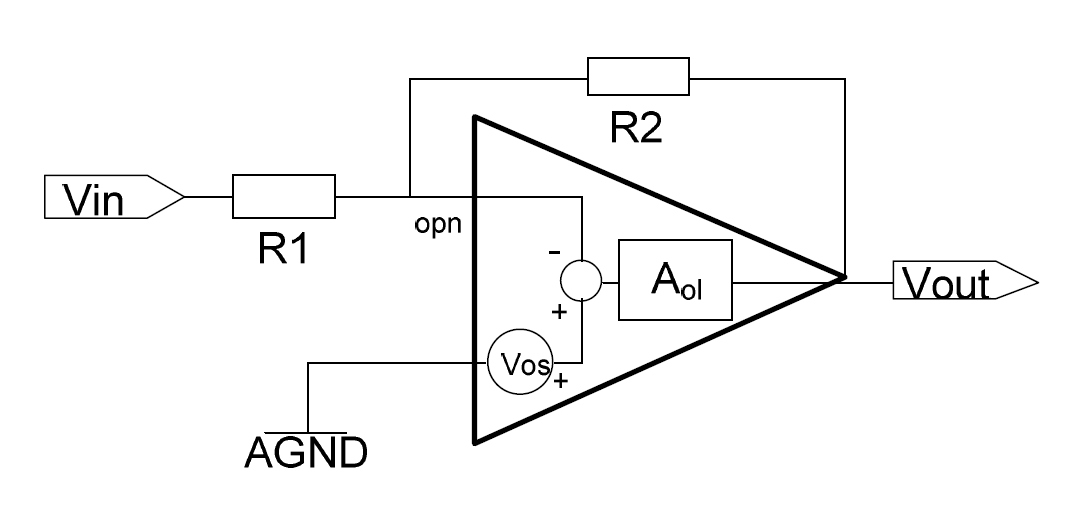
\includegraphics[width=6cm]{./bilder/i-verstaerker.png}
    \end{minipage}\\
\hrule

	\subsubsection{Nichtinvertierender Verstärker}
		\begin{minipage}[T]{13cm}
      Closed-Loop Verst\"arkung
      \hspace{3mm}\fbox{$V_{out} = \frac{A_{ol}}{1+A_{ol}\cdot \frac{R_1}{R_1+R_2}} \cdot V_{in} \cong \left( 1+\frac{R_2}{R_1}\right)  \cdot V_{      in}$}\\
      inkl. Offsetspannung
      \hspace{10.2mm}\fbox{$V_{out} = \frac{A_{ol}}{1+A_{ol}\cdot\frac{R_1}{R_1+R_2}}\cdot(V_{in}+V_{OS})$}\\
      f\"ur $A{ol}$ gross
      \hspace{22mm}\fbox{$V_{out} =\left(1 + \frac{R_2}{R_1}\right) \cdot (V_{in}+V_{OS})$}\\
      Ausgangswiderstand    \hspace{10.5mm}\fbox{$r_{out}=0\Omega$}\\
      Eingangswiderstand    \hspace{11mm}\fbox{$r_{in}=\infty$}\\
    \end{minipage}
		\begin{minipage}{6cm}
      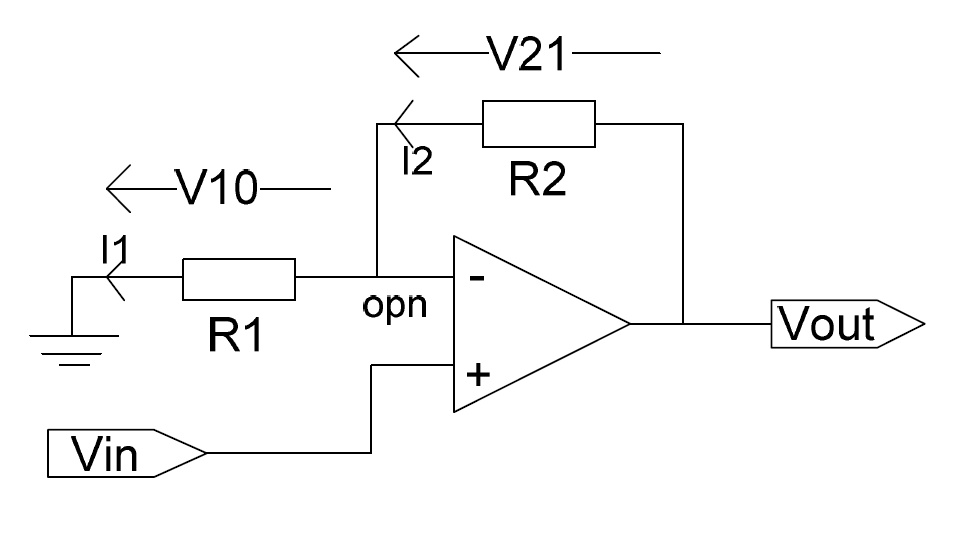
\includegraphics[width=6cm]{./bilder/ni-verstaerker.png}
    \end{minipage}\\
\hrule

  \subsubsection{Invertierender Addierer}
    \begin{minipage}[T]{13cm}
      Closed-Loop Verst\"arkung
      \hspace{3mm}\fbox{$V_{out}= -R_F \cdot \left(V_{in1}\cdot \frac{1}{R_1} + V_{in2}\cdot \frac{1}{R_2}+ \ldots\right) $}\\
      \hspace*{43mm}\fbox{$A_{CL1}=- \frac{R_F}{R_1}$}
      ;\hspace{0.2mm} \fbox{$A_{CL2}=- \frac{R_F}{R_2}$}
      ; \ldots
    \end{minipage}
    \begin{minipage}{6cm}
      \includegraphics[width=6cm]{./bilder/invertadd.png}
    \end{minipage}\\
  
  \hrule
	\subsubsection{Verstärker mit mehreren Eingängen}
		\begin{minipage}[T]{13cm}
      Closed-Loop Verst\"arkung
      \hspace{3mm}\fbox{$V_{out}=-\frac{R_F}{R_1}\cdot V_{in1}-\frac{R_F}{R_2}\cdot V_{in2}+\frac{R_F+(R_1//R_2)}{(R_1//R_2)}\cdot V_{in3}$}\\
      \hspace*{43mm}\fbox{$A_{CL1}=-\frac{R_F}{R_1}$}
      ;\hspace{0.3mm}\fbox{$A_{CL2}=-\frac{R_F}{R_2}$}
      ;\hspace{0.3mm}\fbox{$A_{CL3}=\frac{R_F+(R_1//R_2)}{(R_1//R_2)}$}\\
    \end{minipage}
		\begin{minipage}{6cm}
      \includegraphics[width=6cm]{./bilder/3-eingaenge.png}
    \end{minipage}\\
\hrule

	\subsubsection{Mehrfach-Addierer-Subtrahierer} 		
    \begin{minipage}[T]{13cm}
      1. Man w\"ahlt $R_{F}$\\
      2. Man w\"ahlt $R_{P}$, wobei oft $R_{P}=R_{F}$ gesetzt wird. (optional)\\
      3. $R_{n}=\frac{R_{F}}{\left|A_{n}\right|}$ oder
      $R_{n}=\frac{R_{P}}{\left|A_{n}\right|}$\\ 
      4. Verst\"rkungsbedingung: $A_{N1} +
      \ldots + A_{Nn} = A_{P1} + \ldots + A_{Pn}$ \\Falls unerf\"ullt, muss ein Dummyeingang hinzugefügt werden!
    \end{minipage}
    \begin{minipage}{6cm}
      \includegraphics[width=5.5cm]{./bilder/mehrfach-addierer-subtrahierer.png} 
    \end{minipage}\\
    
 \hrule
  

  \hrule        
	\subsubsection{Gewichteter Subtrahierer}
		\begin{minipage}[T]{13cm}
      Closed-Loop Verst\"arkung
      \hspace{3mm}\fbox{$V_{out}=\frac{R_3}{R_2+R_3}\left(1+\frac{R_F}{R_1}\right)\cdot V_{in2}-\frac{R_F}{R_1}\cdot V_{in1}$}\\
      f\"ur $R_3 = R_F$ und $R_2 = R_1$
      \hspace{0.1mm} \fbox{$V_{out}=\frac{R_F}{R_1}\cdot (V_{in2}-V_{in1})$}
    \end{minipage}
		\begin{minipage}{6cm}
      \includegraphics[width=6cm]{./bilder/gewichtsub.png}
    \end{minipage}\\		
\hrule

	\subsubsection{Differenzverstärker}
    \begin{minipage}[T]{14cm}
      Closed-Loop Verst\"arkung
      \hspace{3mm}\fbox{$V_{out} = \frac{R_3+R_4}{R_3}\cdot \left( \frac{R_1}{R_1+R_2}\cdot V_{ref} + \frac{R_2}{R_1+R_2}\cdot V_{in1}\right)-      \frac{R_4}{R_3}\cdot V_{in2} $}\\
      f\"ur $R_1 = R_3$ und $R_2 = R_4$
      \hspace{1mm} \fbox{$V_{out}= V_{ref} +\frac{R_4}{R_3}\cdot(V_{in1}-V_{in2})$}
    \end{minipage}
    \begin{minipage}{5cm}
      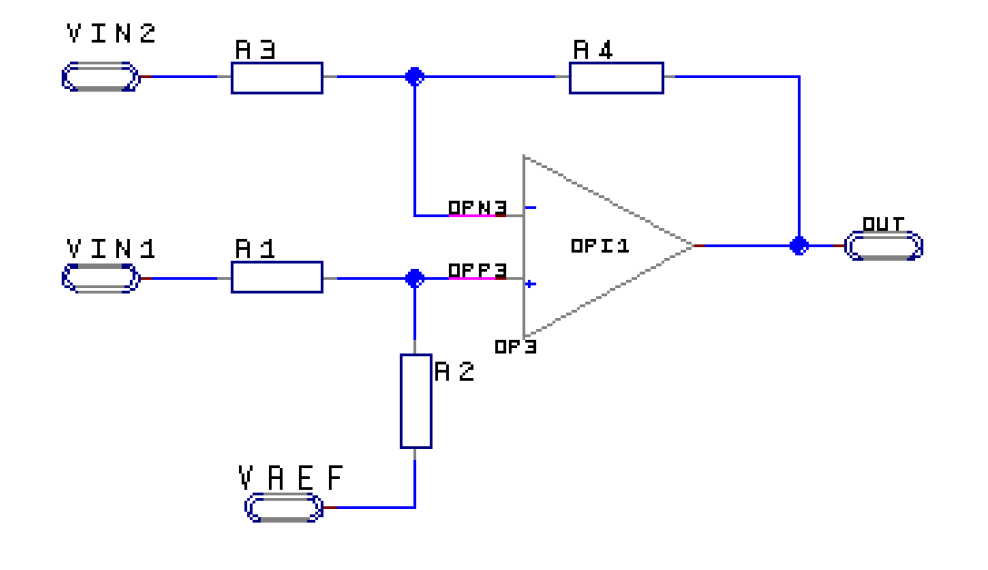
\includegraphics[width=5cm]{./bilder/differenzver.png}
    \end{minipage}\\
\hrule
        
	\subsubsection{Instrumentenverstärker}
		\begin{minipage}[T]{13cm}
      Stufe 1 (Pos Eingang)
      \hspace{18.8mm}\fbox{$V_{opo2} = V_{in2}+ \frac{R_{f2}}{R_G}\cdot(V_{in2}-V_{in1})$}\\
      Stufe 1 (Neg Eingang)
      \hspace{18.3mm}\fbox{$V_{opo1} = V_{in1}- \frac{R_{f1}}{R_G}\cdot(V_{in2}-V_{in1})$}\\
      Stufe 2 Closed-Loop Verst\"arkung
      \hspace{3.4mm}\fbox{$V_{out} = V_{ref}+\frac{R_4}{R_3}\cdot\left(1+\frac{R_{f1}+R_{f2}}{R_G} \right)\cdot (V_{in1}-V_{in2}) $}
		\end{minipage}
    \hspace{0.5cm}
		\begin{minipage}{6cm}
      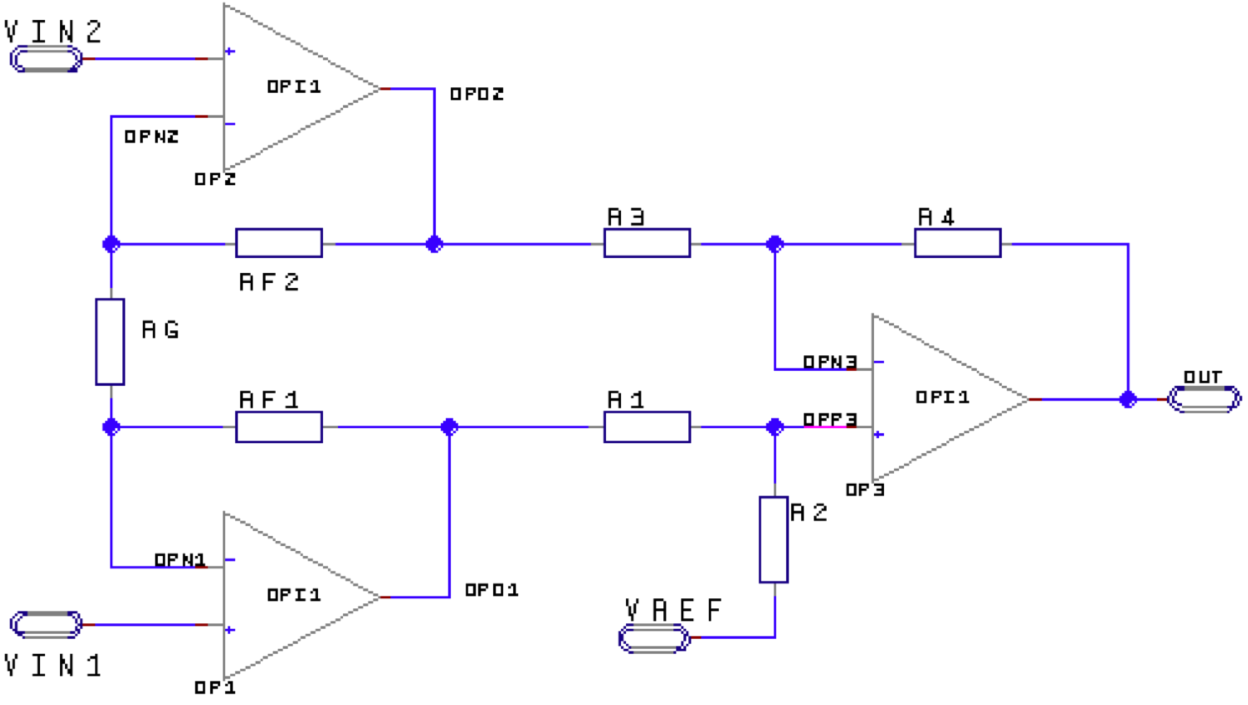
\includegraphics[width=6cm]{./bilder/Instrumentationsverstaerker.png} 
    \end{minipage}\\
  
  \hrule
  \subsubsection{T-Glied in Rückkopplung}
    \begin{minipage}[c]{12cm}
  	 	Für $A \to \infty$ (idealer OP) gilt: \smallskip \\
   	 	\fbox{$v_u=-\frac{R_2 \cdot R_3 + R_2 \cdot R_4 + R_3 \cdot R_4}{R_1 \cdot R_3}$}
   	 	\bigskip \\
   	 	$\Longrightarrow$ hohe Verstärkung mit kleinen Wertunterschieden - 
   	 	z.B.$R_1=R_3=1k\Omega$ und $R_2=R_4=10k\Omega$ ergibt $v_u=-120$ 
   	 	(Vergleich: $v_u=-10$ bei inv. Verstärker) \\
    \end{minipage}
    \hspace{0.5cm}
    \begin{minipage}[c]{5cm}
      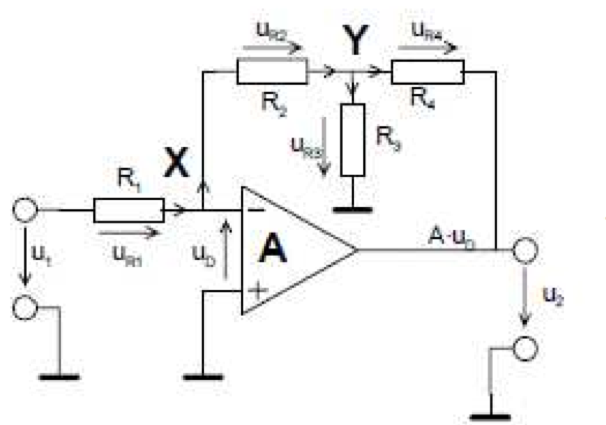
\includegraphics[width=5cm]{./bilder/tglied.png}
    \end{minipage}      

  \hrule 	 
  \subsubsection{Negative Impedance Converter (NIC)}
    \begin{minipage}[c]{12cm}    
      Der Negative Impedance Converter (NIC) stellt einen negativen reellen Widerstand
      dar. Verwendung: Kompensation parasitärer reeller Widerstände. \\
      Nachteil: Masse-Bezug des negativen Widerstands. \bigskip \\
      \fbox{$R_{EQ}=-R \cdot \frac{R_1}{R_2}$}\\
    \end{minipage}
    \begin{minipage}[c]{5cm}
      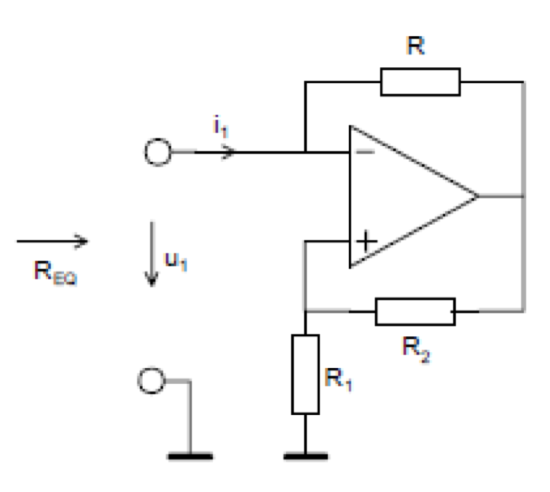
\includegraphics[width=5cm]{./bilder/neg-imp-conv.png}
    \end{minipage}


  \subsubsection{Integrator}
    \begin{minipage}[T]{13cm}
      Closed-Loop Verst\"arkung
      \hspace{3mm}\fbox{$V_{out} =-\frac{1}{R\cdot C} \int{V_{in}}dt + V_{out\hspace{1mm}Anfang}$}\\
      \hspace*{43mm}\fbox{$-\frac{1}{C} \int i_c dt + V_{out\hspace{1mm}Anfang}$}\\
      \hspace*{42mm} \fbox{$\frac{dv_{out}}{dt}=-\frac{v_{in}}{RC}$}\\ \\
      $R_F$ limitiert die Verst\"arkung bei tiefen Frequenzen. D.h. er wirkt als Tiefpass
    \end{minipage} 
    \begin{minipage}{6cm}
      \includegraphics[width=6cm]{./bilder/integrator.png} 
    \end{minipage}\\		
\hrule

  \subsubsection{Differentiator}
    \begin{minipage}[T]{13cm}
      Beim Differentiator gilt $V_{out}=v_N-i_1 \cdot R_F$ wobei $v_N=0$\\
      Closed-Loop Verst\"arkung
      \hspace{3mm}\fbox{$V_{out}=-R_F\cdot C_1 \frac{dv_{in}}{dt}$}\\
      \hspace*{43.2mm}\fbox{$i_1=C_1 \cdot \frac{dv_C}{dt}$}\\
      Die Elemente $C_F$ und $R_1$ sind optional. \\
      Sie beheben jedoch Probleme die ohne \\
      sie entstehen (siehe elemenarer Differentiator). \\
      Mit $C_F$ und $R_1$: \\
      - Keine differentiation bei h\"oheren Frequenzen. \\
      - Limitierte Verst\"arkung bei h\"oheren Frequenzen. \\
      - Eingangswiderstand immer gr\"osser $R_1$ $\rightarrow$ keine Belastung der Signalquelle\\
      - \textbf{Bandpass}-Charakteristik mit $\omega_1 = \frac{1}{R_1C_1}$; $\omega_2 = \frac{1}{R_FC_F}$
    \end{minipage}
    \begin{minipage}{6cm}
      \includegraphics[width=6cm]{./bilder/differentiator.png}
    \end{minipage}\\

  \hrule
  \subsubsection{Buffer (Spannungsfolger / Impedanzwandler)}
    \begin{minipage}[T]{13cm}
      Closed-Loop Verst\"arkung
      \hspace{3mm}\fbox{$V_{out} = \frac{A_{ol}}{1+A_{ol}}\cdot V_{in}\cong V_{in} $}\\
      inkl. Offsetspannung
      \hspace{10.2mm}\fbox{$V_{out} = \frac{A_{ol}}{1+A_{ol}}\cdot(V_{in}+V_{os})\cong V_{in}+V_{os}$}
    \end{minipage} 
    \begin{minipage}{6cm}
      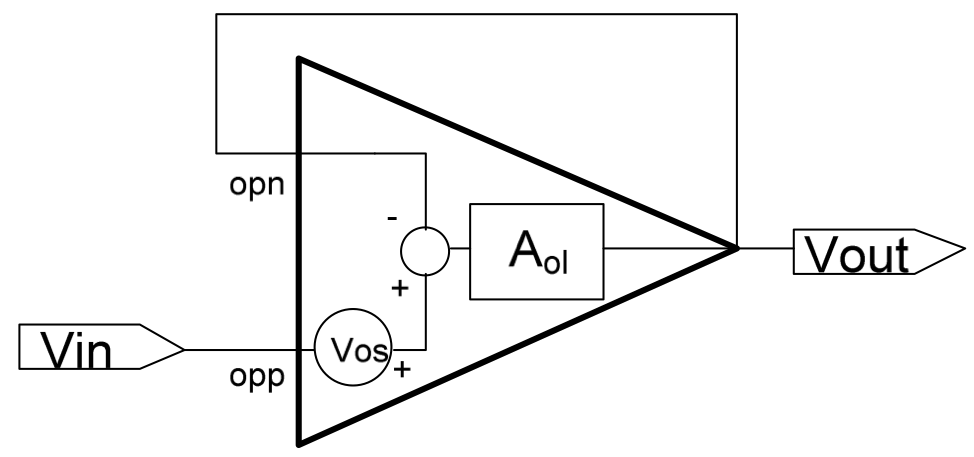
\includegraphics[width=6cm]{./bilder/buffer.png} 
    \end{minipage}\\		
\hrule

\subsection{Schmitt-Trigger}
  \subsubsection{Nicht invertierender Schmitt-Trigger}
		\begin{minipage}[T]{13cm}
      obere Schaltschwelle
      \hspace{10.8mm}\fbox{$V_{T+} = V_{ref}\cdot \frac{R_1+R_f}{R_f}-V_{out_{min}}\cdot\frac{R_1}{R_f}$}\\
      untere Schaltschwelle
      \hspace{9.6mm}\fbox{$V_{T-} = V_{ref}\cdot \frac{R_1+R_f}{R_f}-V_{out_{max}}\cdot\frac{R_1}{R_f}$}\\
      Hysteresespannung
      \hspace{12.8mm}\fbox{$V_{H} = V_{T+}-V_{T-} = (V_{out_{max}}-V_{out_{min}})\cdot\frac{R_1}{R_f}$}\\
    \end{minipage} 
    \begin{minipage}{6cm}
      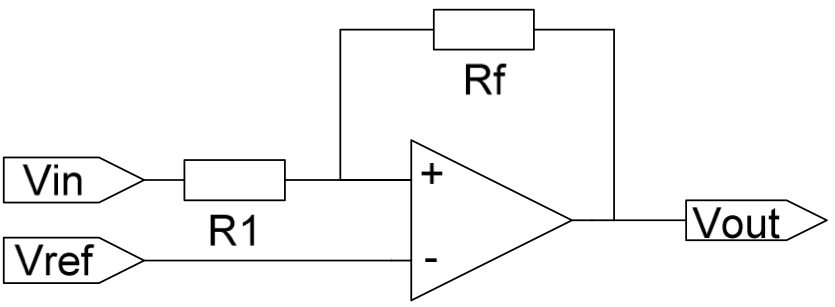
\includegraphics[width=6cm]{./bilder/n-schmitt.png} 
    \end{minipage}\\
            
  \subsubsection{Invertierender Schmitt-Trigger}
    \begin{minipage}[T]{13cm}
      obere Schaltschwelle
      \hspace{10.8mm}\fbox{$V_{T+} = \frac{V_{ref}\cdot R_f+ V_{out_{max}}\cdot R_1}{R_1+R_f}$}\\
      untere Schaltschwelle
      \hspace{9.6mm}\fbox{$V_{T-} = \frac{V_{ref}\cdot R_f+ V_{out_{min}}\cdot R_1}{R_1+R_f}$}\\
      Hysteresespannung
      \hspace{12.8mm}\fbox{$V_{H} = V_{T+}-V_{T-} = (V_{out_{max}}-V_{out_{min}})\cdot\frac{R_1}{R_1+R_f}$}\\ \\
      \textbf{Vorteil}: $V_{in}$ wird nicht unterschiedlich belastet!
    \end{minipage} 
    \begin{minipage}{6cm}
      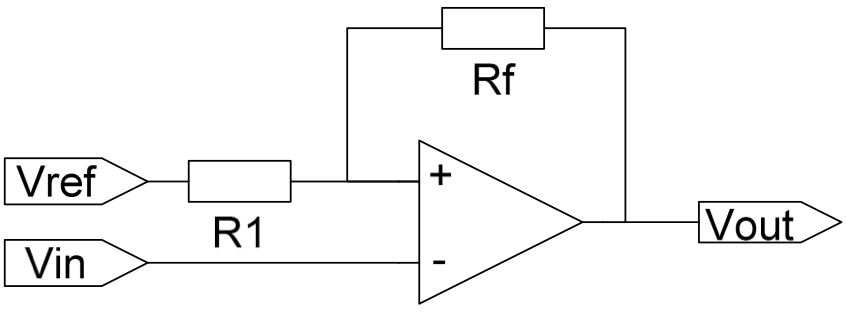
\includegraphics[width=6cm]{./bilder/i-schmitt.png} 
    \end{minipage}\\
            
  \subsubsection{Invertierender Schmitt-Trigger mit freien Schwellen}
    \begin{minipage}[T]{13cm}
      Schaltschwelle
      \hspace{20.8mm}\fbox{$V_{opp} =V_{ref}\cdot \frac{(R_f//R_0)}{R_1 +(R_f//R_0)}+V_{out}\cdot\frac{(R_1//R_0)}{R_f+(R_1//R_0)}$}\\ \\
      $V_{T+} \rightarrow V_{out} = V_{out_{max}} \qquad V_{T-} \rightarrow V_{out} = V_{out_{min}}$ \\
      Dimensionierung des Schmitt-Triggers: (Gegeben: $V_{ref}$, $V_{T+}$, $V_{T-}$)\\
      1. $V_{out_{max}}$ und $V_{out_{min}}$ ermitteln aus Datenblatt (meistens $V_{DD}$, $GND$)\\
      2. $R_f$ w\"ahlen: typisch $100 k\Omega$\\
      3. Widerst\"ande $R_1$ und $R_0$ dimensionieren\\
    \end{minipage} 
    \begin{minipage}{6cm}
      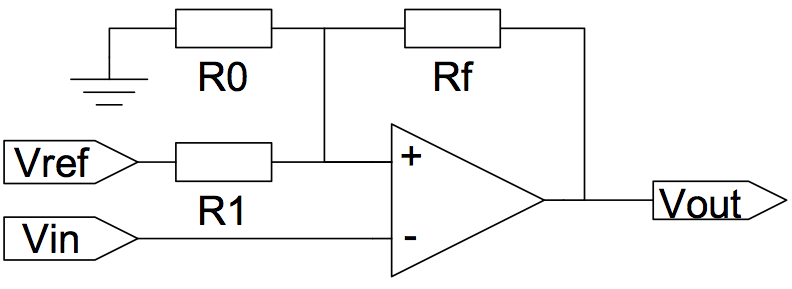
\includegraphics[width=6cm]{./bilder/i-schmittFreieSchwellen.png} 
    \end{minipage}\\
\hrule

\subsection{Gesteuerte Quellen}
  \begin{tabular}{|c|c|c|}
		\hline
		\multirow{2}{*}{Steuergrösse} & \multicolumn{2}{c|}{Ausgangsgrösse}\\ \cline{2-3}
		& V & I \\ \hline
		\multirow{8}{*}{V}	& Spannungsgesteuerte Spannungsquelle	& Spannungsgesteuerte Stromquelle		\\
    & \bf{VCVS} & \bf{VCCS} \\
		& Voltage Controlled Voltage Source		& Voltage Controlled Current Source \\ \cline{2-3}
		& 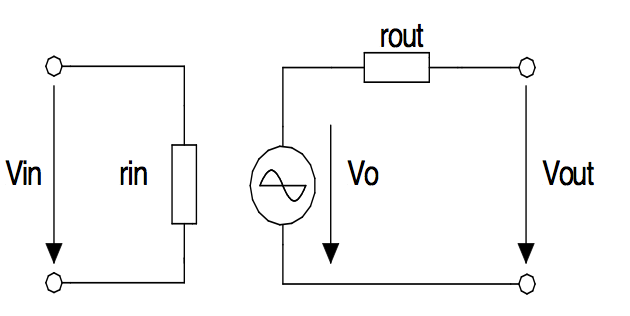
\includegraphics[width=4cm,trim=0 0 0 -5]{./bilder/vcvs.png}	
		& 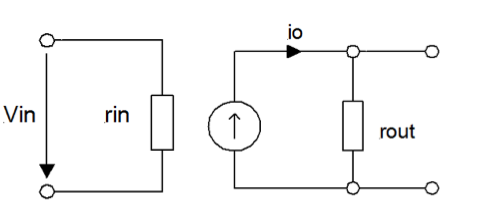
\includegraphics[width=4cm,trim=0 0 0 -5]{./bilder/vccs.png}  \\ \cline{2-3}
		& $v_{out}=v_{in} \cdot A_v$ & $i_{out} = v_{in} \cdot g_m$ \\
		& $A_v$: Spannungsverstärkung & $g_m$: Transkonduktanz  \\ \cline{2-3}
		& 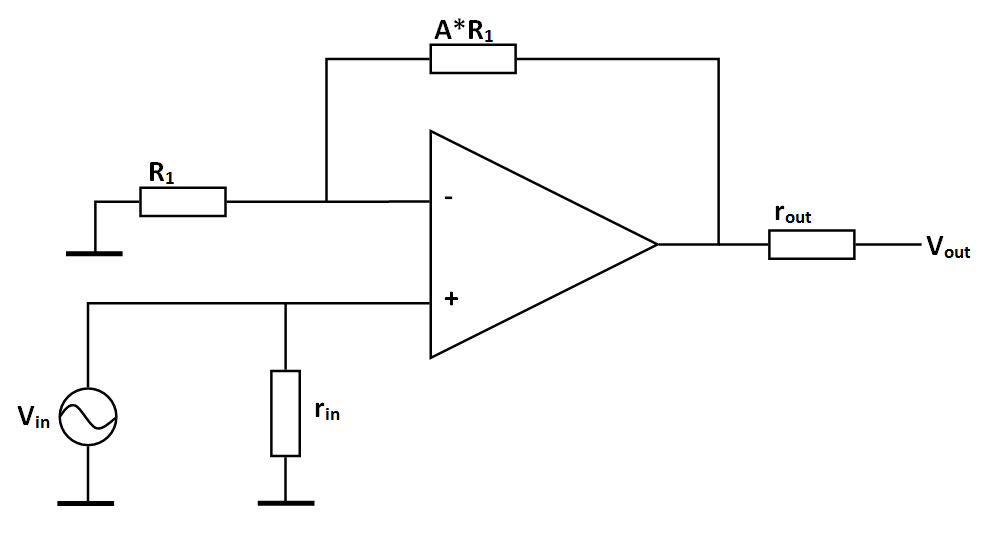
\includegraphics[width=4cm,trim=0 0 0 -5]{./bilder/vcvs_schaltung.png}
		& 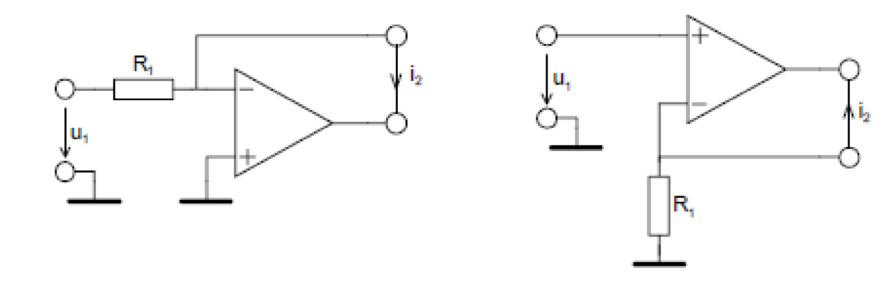
\includegraphics[width=4cm,trim=0 0 0 -5]{./bilder/vccs_schaltung.png}  \\
		&	& $I_2=\frac{V_1}{R_1}$ bzw. $I_2=-\frac{V_1}{R_1}$\\ 	\hline	
		\multirow{8}{*}{I}	& Stromgesteuerte Spannungsquelle		& Stromgesteuerte Stromquelle \\
		& \bf{CCVS} & \bf{CCCS} \\
		& Current Controlled Voltage Source	& Current Controlled Current Source \\ \cline{2-3}
		& 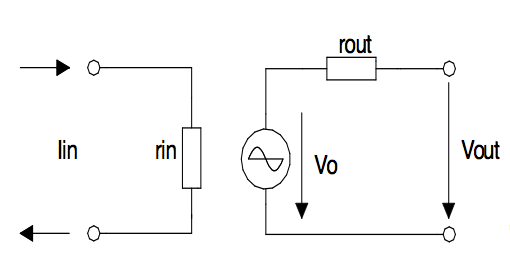
\includegraphics[width=4cm,trim=0 0 0 -5]{./bilder/ccvs.png}	
		& 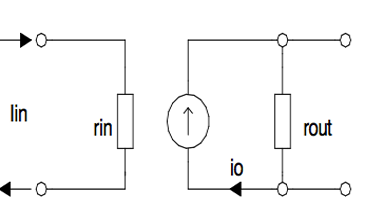
\includegraphics[width=4cm,trim=0 0 0 -5]{./bilder/cccs.png}  \\ \cline{2-3}
		& $v_{out}=i_{in} \cdot r_m$  & $i_{out} = i_{in \cdot A_i}$  \\
		& $r_m$: Transimpedanz  & $A_i$: Stromverstärkung \\ \cline{2-3}
		& 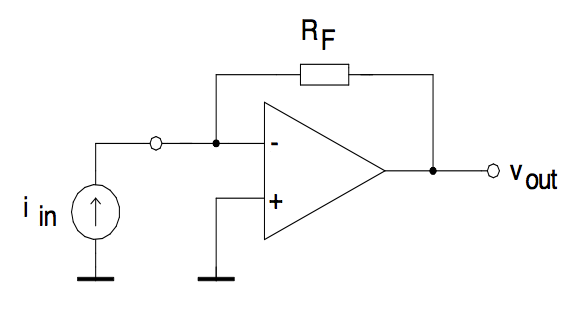
\includegraphics[width=4cm,trim=0 0 0 -5]{./bilder/tia.png}
		& 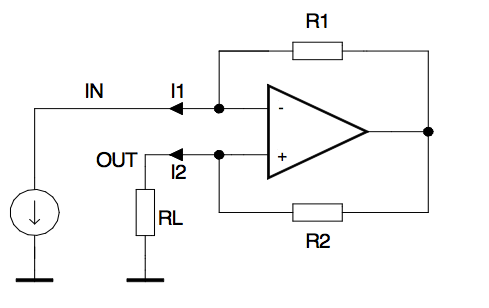
\includegraphics[width=4cm,trim=0 0 0 -5]{./bilder/cccs-schaltung.png}		\\ 
		& $v_{out}=-i_{in} \cdot r_F$ & $A_i=\frac{I_2}{I_1}=\frac{R_1}{R_2}$	\\ \hline
	\end{tabular} \\


\subsection{Nichtidealit\"aten des Operationsverst\"arkers}
  \subsubsection{Eingangsstromkompensation (Bias-Strom) ohne AC-Zweige (Kondensatoren)}
    \begin{minipage}[b]{6cm}
      \includegraphics[height=3cm]{./bilder/spannungsfolger.png}\\
      {\bf Spannungsfolger}\\ \\
      $R_2$ sei ein gegebener Quellenwiderstand\\
      $R_F$ muss eingefügt werden\\ \\
      \fbox{$R_F=R_2$}
    \end{minipage}\hfill
    \begin{minipage}[b]{6cm}
      \includegraphics[height=3cm]{./bilder/nichtinver}\\
      {\bf Nichtinvertierender Verstärker}\\ \\
      Hier sei der Quellenwiderstand vernachl\"assigbar.\\ 
      $R_2$ muss eingefügt werden\\ \\
      \fbox{$R_2=R_F//R_1$}
    \end{minipage}\hfill
    \begin{minipage}[b]{6cm}
    \includegraphics[height=3cm]{./bilder/inver}\\
      {\bf Invertierender Verstärker}\\ \\ \\ \\
      $R_2$ muss eingefügt werden\\ \\
      \fbox{$R_2=R_F//R_1$}
    \end{minipage}
    
    \begin{tabular}{p{7cm} l}
      \textbf{Ausgangsspannungsfehler} auf Grund des nicht 
      kompensierbaren \textbf{Offsetstroms} (nur bei Kompensation): &
      \begin{tabular}{l l}
        \fbox{$V_{out \hspace{1mm}E}=R_F\cdot (I_N-I_P) = R_F \cdot \left|I_{OS}\right|$}  &
        mit Eingangsstromkompensation \\
        \fbox{$V_{out \hspace{1mm}E}= R_F \cdot \left|I_N\right|$} &
        ohne Eingangsstromkompensation
      \end{tabular} \\
    \end{tabular}
    \begin{tabular}{l l l}
      \textbf{Bias Strom} & \fbox{$I_B = \frac{I_P + I_N}{2}$} & ist kompensierbar \\
      \textbf{Offset-Strom} & \fbox{$I_{OS}= \left| I_P - I_N \right|$} & nicht kompensierbar
    \end{tabular}
    

	\subsubsection{Zusammenfassung aller Fehlereinflüsse}
    \begin{minipage}[T]{12.5cm}
      \underline{{\bf Gleichtaktunterdr\"uckung} Common-Mode-Rejection Ratio $CMRR$}\\
            
      Offsetspannung
      \hspace{18.3mm}\fbox{$V_{OS}=\frac{V_{CM}}{CMRR_{lin}}$} mit \fbox{$V_{CM} = V_{opp} = V_{opn}$}\\
      Lineare Definition
      \hspace{14.2mm}\fbox{$CMRR_{lin}=\frac{dV_{CM}}{dV_{OS}}=10^{\frac{CMRR_{dB}}{20}}$}\\
      Logarithmische Definition
      \hspace{2.2mm}\fbox{$CMRR_{dB}=20 \cdot log(CMRR_{lin})=20 \cdot log\left( \frac{dV_{CM}}{dV_{OS}}\right) $}\\
      Ausgangs-Fehlerspannung
      \hspace{2.2mm}\fbox{$V_{out \hspace{1mm} E}=\left|V_{OS}\right| \cdot A_{CL+}=\left| \frac{\Delta V_{CM}}{CMRR_{lin}}\right|A_{CL+}$}
            
      \vspace{2mm}
      \underline{{\bf Power-Supply-Unterdrückungs-Fehler} Power-Supply-Rejection Ratio $PSRR$}\\
            
      Offsetspannung
      \hspace{18.3mm}\fbox{$V_{OS}=\frac{\Delta V_{Supply}}{PSRR_{lin}}$}\\
      Lineare Definition
      \hspace{14.2mm}\fbox{$PSRR_{lin}=\frac{dV_{Supply}}{dV_{OS}}=10^{\frac{PSRR_{dB}}{20}}$}\\
      Logarithmische Definition
      \hspace{2.2mm}\fbox{$PSRR_{dB}=20\cdot log(PSRR_{lin})=20\cdot log\left( \frac{dV_{Supply}}{dV_{OS}}\right) $}\\
      Ausgangs-Fehlerspannung
      \hspace{2.2mm}\fbox{$V_{out \hspace{1mm}E}=\left|V_{OS}\right| \cdot A_{CL+}=\left| \frac{\Delta V_{Supply}}{PSRR_{lin}}\right| A_{CL+}$}\\
            
      \vspace{2mm}
      \underline{\bf Gesamtfehlerspannung}\\
            
      \hspace*{43.3mm}\fbox{$V_{out\hspace{1mm}E\hspace{1mm}total}=A_{CL+}\cdot\left[\left|V_{OS}\right|+\frac{\left|V_{CM}\right|}{CMRR}+\frac{      \left|\Delta V_{Supply}\right|}{PSRR}\right]+\left|I_{OS}\right|\cdot R_F$}\\
    \end{minipage}
    \begin{minipage}[b]{6.5cm}
      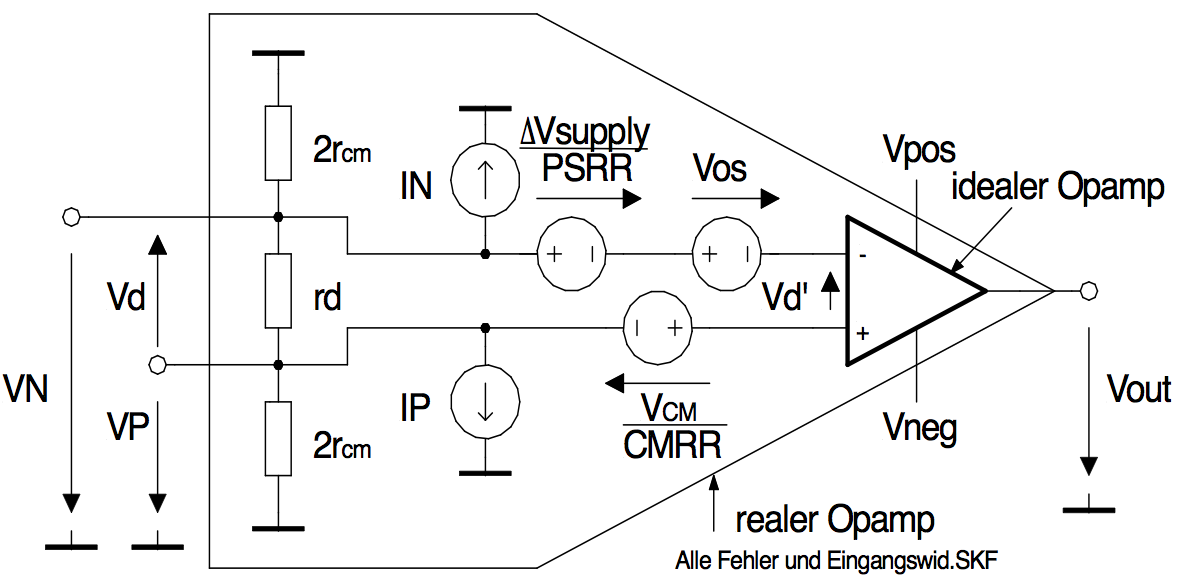
\includegraphics[width=6.5cm]{./bilder/OPAmpAlleFehler}
    \end{minipage}
\hrule
\hrule
\begingroup
  \let\clearpage\relax
  \section{Halbleiter}
\subsection{pn-Übergang}
  \begin{minipage}{14cm}
    N-Schicht wird mit Phosphor dotiert, dadurch entsteht ein Elektron welches schwächer gebunden ist.
    P-Schicht wird mit Bor dotiert, dadurch hat ein Si-Atom eine unaufgefüllte Schale. \\ \\
    Durch Anlegen einer \textbf{positiven} Spannung an der P-Zone, wird die Raumladungszone (RLZ) schmaler. 
    Dadurch wird der pn-Übergang leitend.\\
    Durch Anlegen einer \textbf{negativen} Spannung an der P-Zone, wird die Raumladungszone breiter. 
    Der pn-Übergang sperrt.
  \end{minipage}
  \begin{minipage}{5cm}
    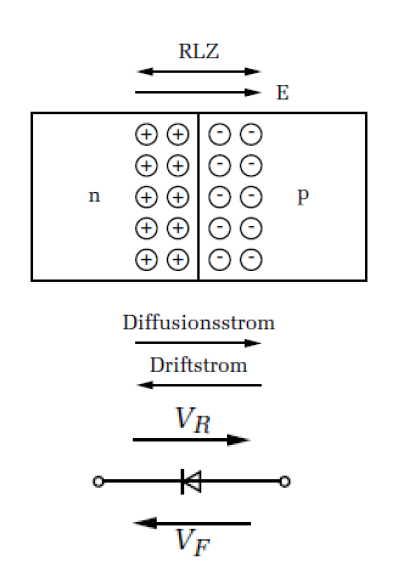
\includegraphics[width=5cm]{./bilder/pn_uebergang.png}
  \end{minipage}

\subsection{Diode}
  \underline{\bf Temperaturverhalten}\\
  Thermospannung
  \hspace{15.3mm}\fbox{$V_T = \frac{k_B\cdot T}{q}$} $V_{T_{23^\circ C}} = 25.5 mV$ \fbox{$k_B=1.38065 \cdot 10^{-23}$ J/K; $q=1.6021765 \cdot 10^  {-19}$ C; $T$=Temp [K]}\\
  \begin{minipage}[T]{8cm}
    {\bf Sperrbetrieb}\\
    $U_{np} > 5.7V$: Temp-Koeff: $+2 mV/K$\\
    $U_{np} < 5.7V$: Temp-Koeff: $-0.5 mV/K$\\
  \end{minipage}
  \begin{minipage}{5cm}
    {\bf Durchlassbetrieb}\\
    Temp-Koeff: $-2 mV/K$\\
    typisch $U_{F0} = 0.6V$
  \end{minipage}
  \begin{minipage}{6cm}
    Verdoppelung des Sperrstroms bei einer Temperaturerhöhung von $10^\circ C$
  \end{minipage}
            
  \underline{\bf Strom-Spannungs-Verhalten}\\
  \begin{minipage}[T]{8.5cm}
    Vorw\"artsstrom $I_f$
    \hspace{14.6mm}\fbox{$I_f = I_S\cdot \left(e^\frac{V_f}{m\cdot V_T} -1\right)$}\\
  \end{minipage}
  \begin{minipage}{7cm}
    $I_S$=S\"attigungssperrstrom ($<$ pA)\\
    $m$= Emissionskoeff. ($1<m<2$, meist ca. 1)\\
    $V_T$=Thermospannung
  \end{minipage}
  \begin{minipage}{3.5cm}
    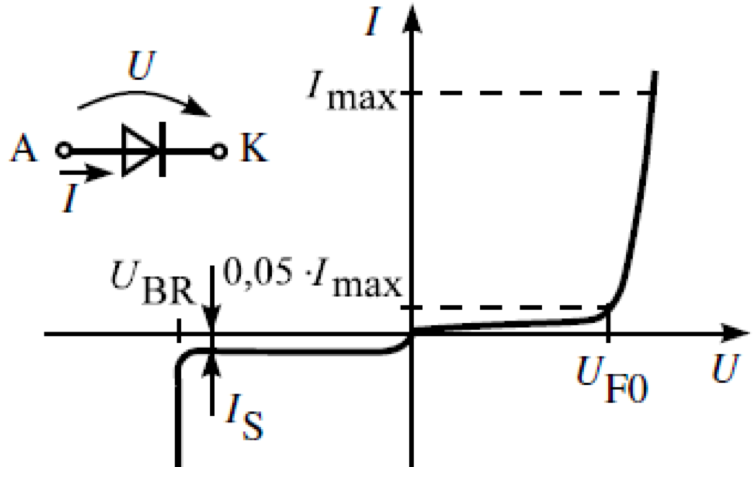
\includegraphics[width=3.5cm]{./bilder/IU_Kennlinie_Diode}\\
  \end{minipage}
  gilt für $V_f \leq U_{F0}$ (sperrend). Für $V_f \geq U_{F0}$ ist die Kurve linear (leitend).\\

  \begin{minipage}[T]{9.5cm}
    Sperrstrom $I_{SP}$
    \hspace{18mm}\fbox{$I_{SP}(T) = I_{SP}(T_0)\cdot e^{C_R\cdot(T-T_0)}$}\\
    temperaturabh\"angig
    \hspace{11mm}\fbox{$C_{R_{Si}} = \frac{W_g}{2\cdot k_B\cdot T_0^2} \cong 0.07 K^{-1}$}\\
  \end{minipage}
  \begin{minipage}{6cm}
    $T_0 = 300K$\\
    $C_{R_{Si}}$ (f\"ur Silizium bei Raumtemp.)\\
    $W_g$ Energie
  \end{minipage}
  \begin{minipage}{3.5cm}
    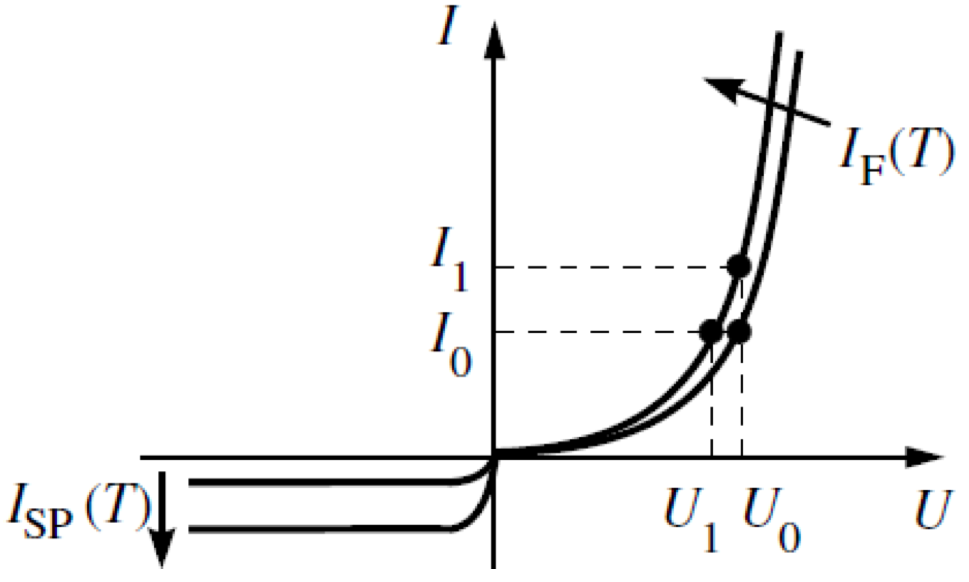
\includegraphics[width=3.5cm]{./bilder/IspKennlinieDiodeTemp}\\
  \end{minipage}\\
  {\bf Faustregel:} Verdoppelung des Sperrstroms bei einer Temperaturerh\"ohung um $10 ^\circ C$
            
  \begin{minipage}[T]{8.5cm}
    Grosssignalwiderstand
    \hspace{8mm}\fbox{$R_D = \frac{V_0}{I_0}$}\\
    Kleinsignalwiderstand
    \hspace{8.4mm}\fbox{$r_d = \frac{mV_T}{I_0} = \frac{dV}{dI}$}\\
  \end{minipage}
  \begin{minipage}{5cm}
    $V_0$= Arbeitspunkt-Spannung\\
    $I_0$= Arbeitspunkt-Strom\\
    $V_T$=Thermospannung
  \end{minipage}
  \begin{minipage}{5.5cm}
    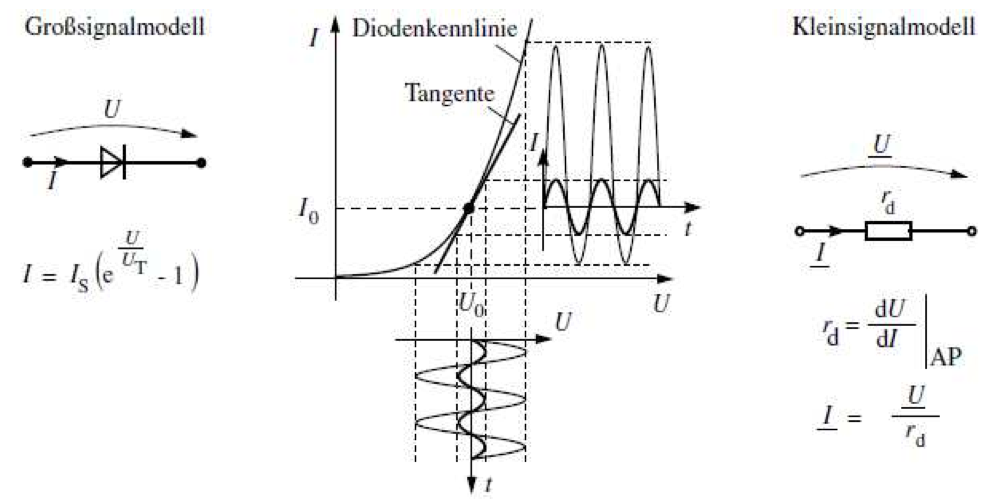
\includegraphics[width=5.5cm]{./bilder/GrossKleinSig}\\
  \end{minipage}
  
        

  \begin{minipage}[T]{15.5cm}
    \underline{\bf Kleinsignalersatzschaltbild}\\
    $R_B$: Bahnwiderstand (Zuleitung, Kontaktierung) : gerader Verlauf der Kennlinie ab $U_f >0.6V$\\
    $r_d$: differentieller Widerstand des pn-\"Ubergangs\\
    $C_D$: Diffusionskapazit\"at bei positiver Diodenspannung\\
    $C_S$: Sperrschichtkapazit\"at bei negativer Diodenspannung\\
  \end{minipage}
  \begin{minipage}{3.5cm}
    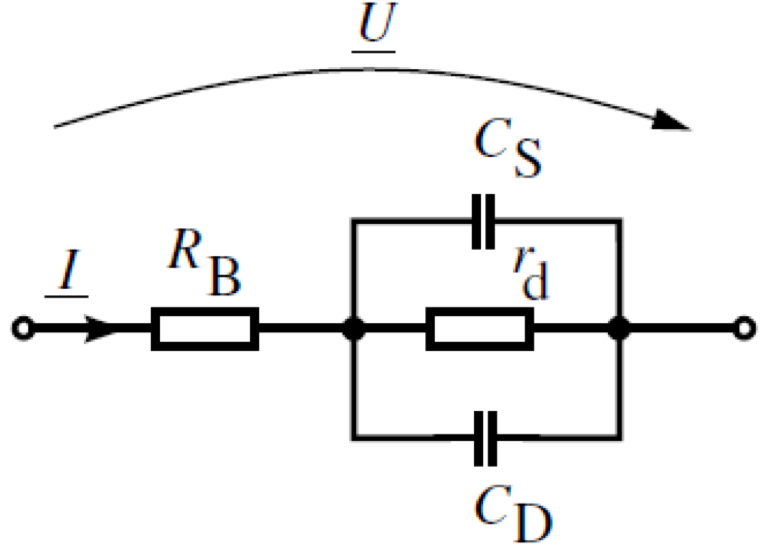
\includegraphics[width=3.5cm]{./bilder/DiodeKleinsigErs}\\
  \end{minipage}\\
  
  \hrule
  \vspace{1mm}
   \begin{minipage}[t]{9cm}
    \underline{\bf Zener-Diode}\\
    $I_{Z0} \approx 0.05 \cdot I_{Zmax}$\\
    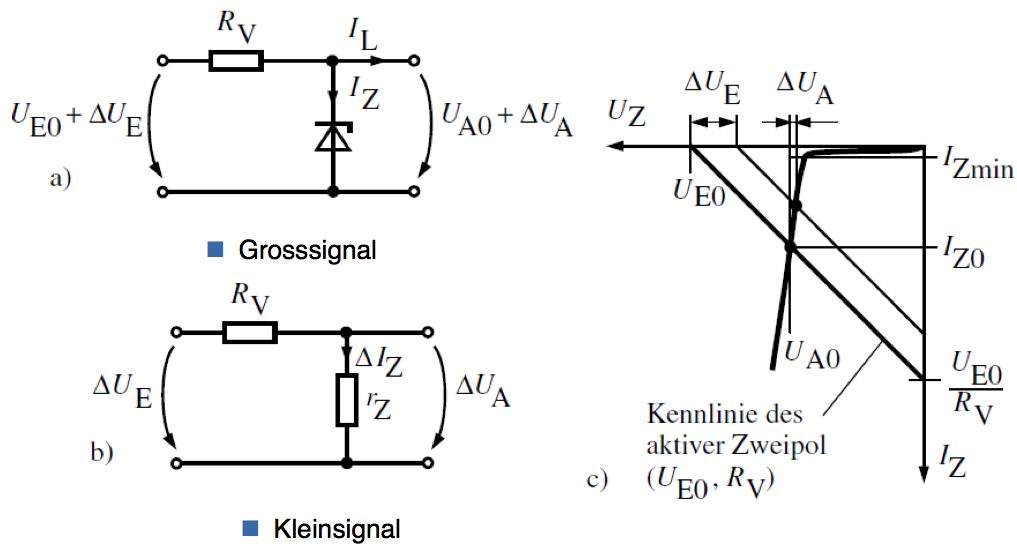
\includegraphics[height=4cm]{./bilder/ZDiodeEig} 
  \end{minipage}
  \begin{minipage}[t]{9cm}
    \underline{\bf Kapazit\"atsdiode (Varicap)}\\
    \begin{minipage}[t]{4.9cm}
      \fbox{$C_S = C_{S0} \cdot\left(1+ \frac{U_{SP}}{U_D}\right)^{-q}$}\\\\
      $q \cong 0.5$\\
      $U_{SP}$: gew\"ahlte Sperrspannung\\
      $C_S$: resultierende Kapazit\"at
    \end{minipage}
    \begin{minipage}{4cm}
      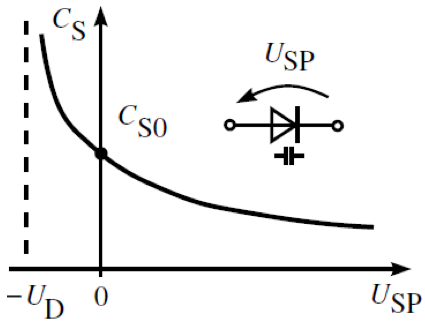
\includegraphics[width=4cm]{./bilder/CDiodeEig}
    \end{minipage}
  \end{minipage}\\
  
\hrule

  \section{Transistoren}
\subsection{Übersicht Transistoren}
  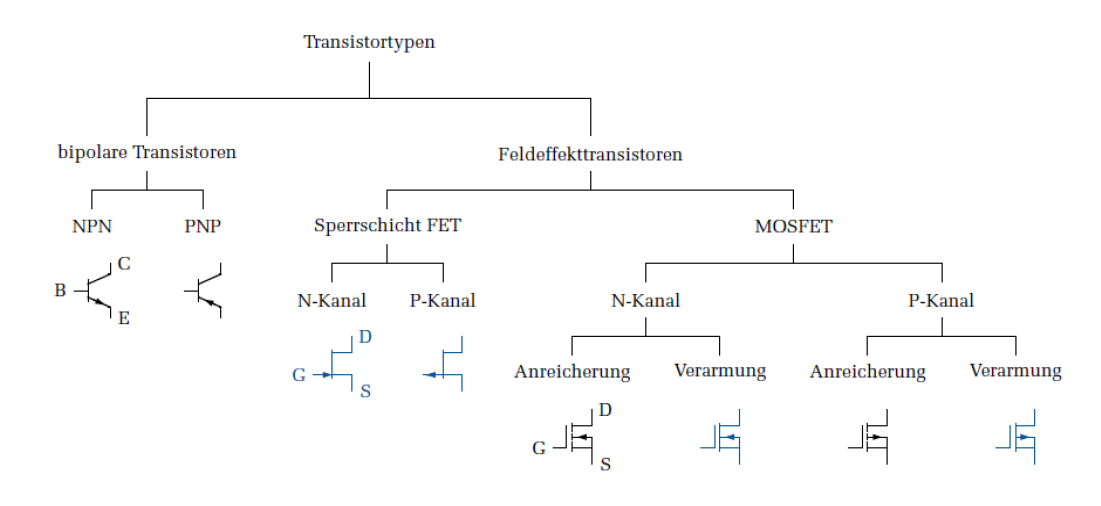
\includegraphics[width=12cm]{./bilder/transistoren_uebersicht.png}
\subsection{Bipolar-Transistor}
  \subsubsection{Ebers-Moll-Ersatzschaltbild}
    \begin{minipage}[T]{16cm}
      Kollektorstrom
      \hspace{18.7mm}\fbox{$I_C = A_N\cdot I_{ES} \cdot\left(e^{\frac{U_{BE}}{U_T}}-1\right) - I_{CS}\cdot\left( e^{\frac{U_{BC}}{U_T}}-1\right)       = A_N \cdot I_{ED} - I_{CD}$}\\
      Emitterrstrom
      \hspace{19.7mm}\fbox{$I_E = I_{ES} \cdot\left(e^{\frac{U_{BE}}{U_T}}-1\right) - A_I\cdot I_{CS}\cdot\left( e^{\frac{U_{BC}}{U_T}}-1\right)      = I_{ED} - A_N \cdot I_{CD}$}\\
    \end{minipage}
    
    \begin{minipage}[T]{13cm}
      Basisstrom
      \hspace{25.1mm}\fbox{$I_B = I_E - I_C$}\vspace{1mm}\\ 
      \hspace*{43mm}$I_{ES}/I_{CS}$: S\"attigungssperrstrom von Emitter/Kollektor\\
      \hspace*{43mm}$U_T$: Thermospannung\\
      \hspace*{43mm}$A_N / A_I$: Verst\"arkungsfaktoren\\
      \hspace*{43mm}$I_{ED}/I_{CD}$: Diodenvorw\"artsstr\"ome (siehe Diode)\\
    \end{minipage}
    \begin{minipage}[T]{6cm}
      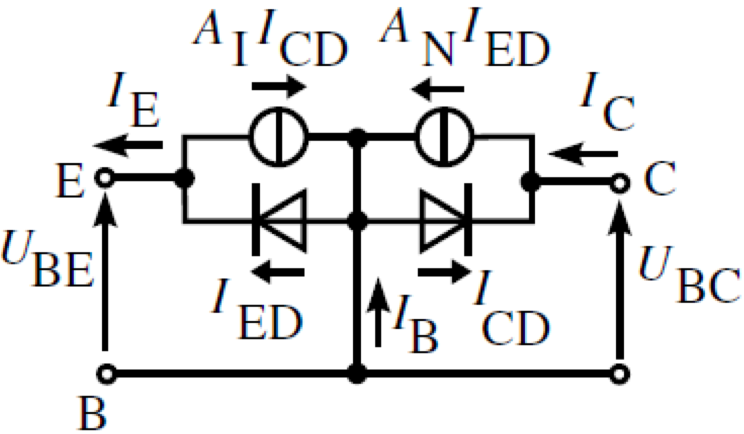
\includegraphics[width=6cm]{./bilder/EberMollModell.png}
    \end{minipage}
            
  \subsubsection{Stromverst\"arkungsfaktoren}
    \begin{minipage}[T]{6cm}
      \bf Basisschaltung\\
      \fbox{$A_N = \frac{I_C}{I_E}$}\\
      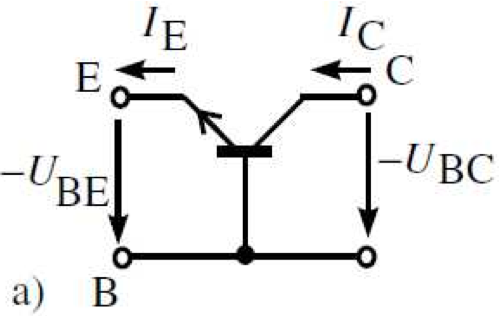
\includegraphics[height=2.3cm]{./bilder/AmpBasisSch.png}
    \end{minipage}
    \begin{minipage}[T]{6cm}
      \bf Emitterschaltung\\
      \fbox{$B_N = \frac{I_C}{I_B} = \frac{A_N}{1-A_N}$}\\
      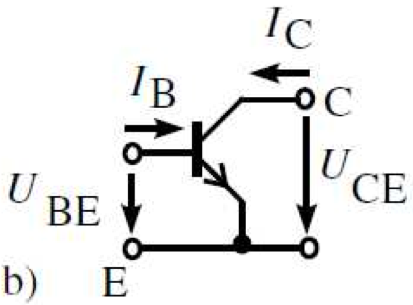
\includegraphics[height=2.3cm]{./bilder/AmpEmitSch.png}                
    \end{minipage}
    \begin{minipage}[T]{6cm}
      \bf Kollektorschaltung\\
      \fbox{$C_N = \frac{I_E}{I_B} = \frac{1}{1-A_N}$}\\
      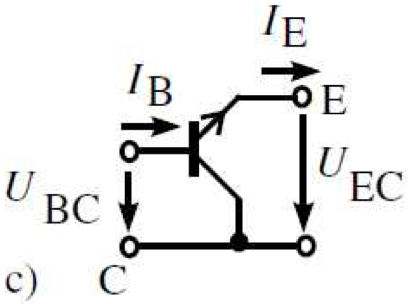
\includegraphics[height=2.3cm]{./bilder/AmpKolSch.png}                
    \end{minipage}
    
\hrule

  \subsubsection{Kennlinienfelder}
    \begin{minipage}[T]{14cm}
      {\bf Ausgangskennlinie (I) $I_C(V_{CE})$}\\
      typ.: $V_{CE_{sat}}=0.3V$ und Ausgangswiderstand \fbox{$r_{CE} \cong \frac{V_{Early}}{I_{C0}}$}\\
      mit berücksichtigung des Early-Effekts gilt 
      \fbox{$I_C = (B_N\cdot I_B + I_{CE0})\left(1+\frac{U_{CE}}{U_{Early}}\right)$}
      \hrule\vspace{1mm}
      {\bf Strom\"ubertragungskennlinie (II) $I_C(I_B)$}\\
      Kollektorstrom: $I_C = \frac{A_N}{1-A_N}\cdot I_B + \frac{A_N\cdot (1-A_I)}{1-A_N}\cdot I_{CS} = B_N\cdot I_B + I_{CE0} \cong B_N\cdot I_B$\\
      \hrule\vspace{1mm}
      {\bf Eingangskennlinie (III)}\\
      Basisstrom: $I_B = I_{ES}\cdot\left(e^{\frac{V_{BE}}{V_T}}-1\right)$\\
      Kleinsignalwiderstand: \fbox{$r_{BE} = \frac{m\cdot V_T}{I_{B0}} = \frac{dV_{BE}}{dI_B}$} mit $I_{B0}$: Arbeitspunktstrom\\
      \hrule\vspace{1mm}
      {\bf Spannungsr\"uckwirkungskennlinie (IV)}\\
      $V_{BE} = \eta \cdot V_{CE}$ mit $\eta \cong 0.1 \%$ (kann meist vernachl\"assigt werden!)\\
    \end{minipage}
    \begin{minipage}[T]{5cm}
      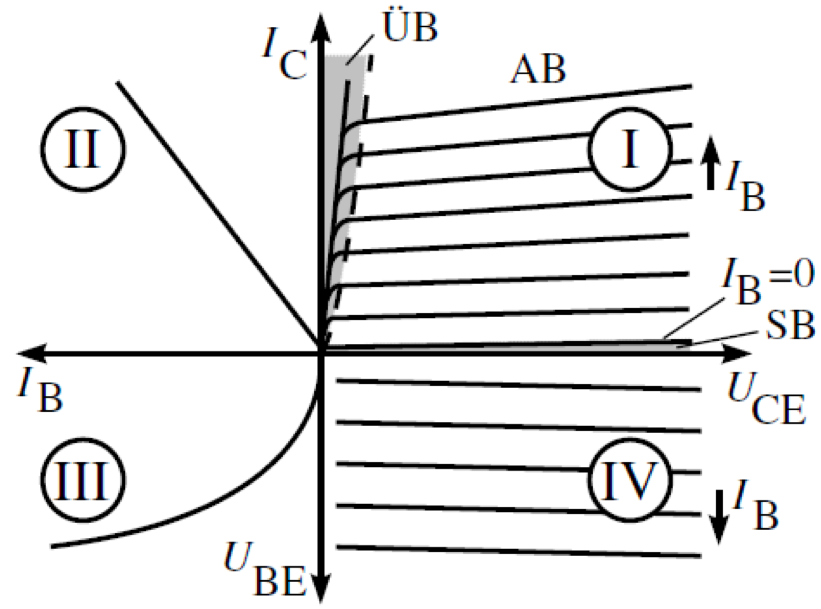
\includegraphics[width=5cm]{./bilder/BipTraKennlinien.png}\\
      ÜB: Übersteuerungsbereich\\
      AB: Arbeitsbereich\\
      SB: Sperrbereich
    \end{minipage}
    


  \subsubsection{Kleinsignal-Modell}
    \begin{minipage}[T]{14cm}
      \begin{tabular}{p{3.5cm} l}
        Eingangswiderstand & 
        \fbox{$r_B =h_{11e} = \left.\frac{dU_{BE}}{dI_B}\right|_{U_{CE0}} = \frac{U_T}{I_{B0}} $}\\
     
        Spannungsrückwirkung & 
        \fbox{$\eta=h_{12e} = \left.\frac{dU_{BE}}{dU_{CE}}\right|_{I_{B0}} \approx 0$}\\
        %
        Stromverst\"arkung & 
        \fbox{$b = h_{FE} = \left.\frac{IC}{I_B}\right|_{U_{CE0}} =B_N\cdot\left(1+\frac{U_{CE0}}{U_{Early}}\right) \approx B_N$}\\
        %
        Ausgangswiderstand &
        \fbox{$r_{CE} = \left.\frac{dU_{CE}}{dI_C}\right|_{I_{B0}} \cong \frac{U_{EA}}{I_{C0}}$}\\
        
        Steilheit &
        \fbox{$S = \frac{b}{r_{BE}} = \frac{I_{C0}}{m\cdot V_T} = g_m = \frac{dI_{OUT}}{dV_{IN}}$}\\
        
        
      \end{tabular}
    \end{minipage}
    \begin{minipage}[T]{5cm}
      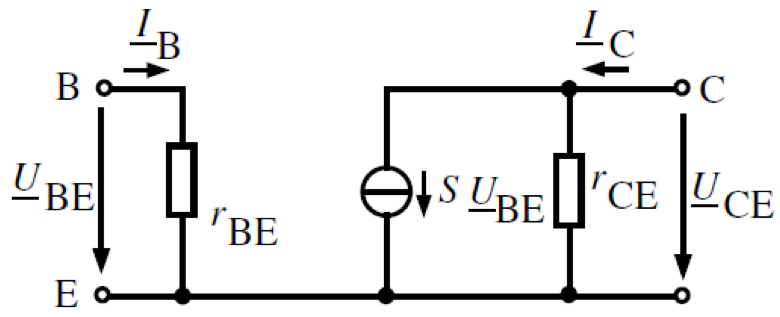
\includegraphics[width=5cm]{./bilder/BipTraErsatzsch.png}\\
      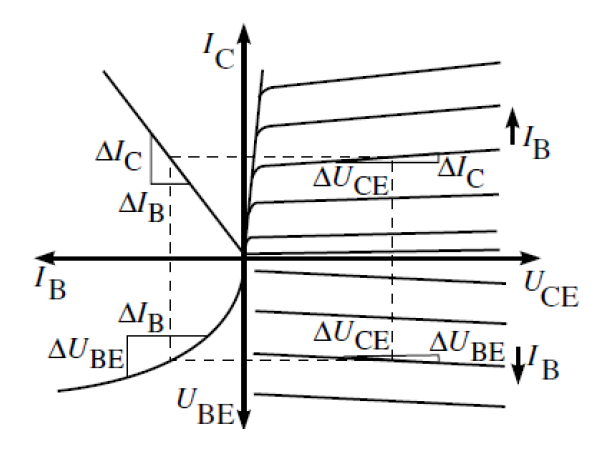
\includegraphics[width=5cm]{./bilder/KleinSigMod.png}
    \end{minipage}
            
  \subsubsection{Kleinsignal-Ersatzschaltung der Emitterschaltung}
    \begin{minipage}[T]{14cm}
      Ausgangsspannung
      \hspace{13mm}\fbox{$U_a = -b\cdot I_B\cdot(R_C // r_{CE})$}\\
      Basisstrom
      \hspace{25.3mm}\fbox{$I_B = \frac{U_e}{r_{BE}}$}\\
      Verst\"arkung
      \hspace{23.3mm}\fbox{$V_U = \frac{U_a}{U_e} = -\frac{b}{r_{BE}}\cdot(R_C//r_{CE}) = -S\cdot(R_C//r_{CE})$}\\
    \end{minipage}
    \begin{minipage}[T]{5cm}
      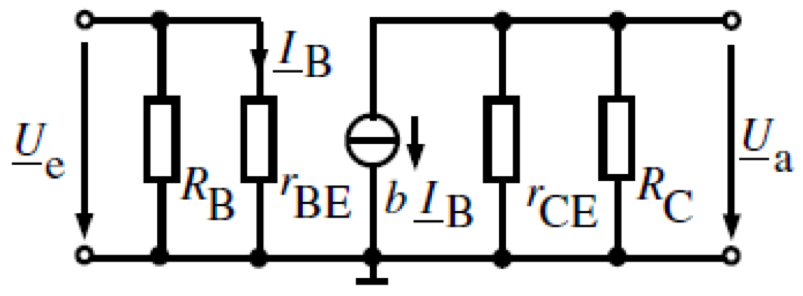
\includegraphics[width=5cm]{./bilder/KleinSigErsEmmitersch.png}
    \end{minipage}
            
    \subsubsection{Frequenzabh\"angigkeit des Bipolartransistors}
      \begin{minipage}[T]{11cm}
        Stromverst\"arkung
        \hspace{14.5mm}\fbox{$h_{21e}(\omega)\approx \frac{b}{1+ \jmath\omega\cdot r_{BE}\cdot (C_E + C_{BE)}}$}\\
        bei $\omega$ = Transitfrequenz $\omega_T$ ist die Stromverst\"arkung $h_{21e} = 1$\\
        Transitfrequenz wird ebenfalls als Gain-Bandwith-Product GBP\\bezeichnet.
        $\omega_1 = \omega_T = b\cdot \omega_{\beta} \approx \omega_{\alpha}$
      \end{minipage}
      \begin{minipage}[T]{8cm}
        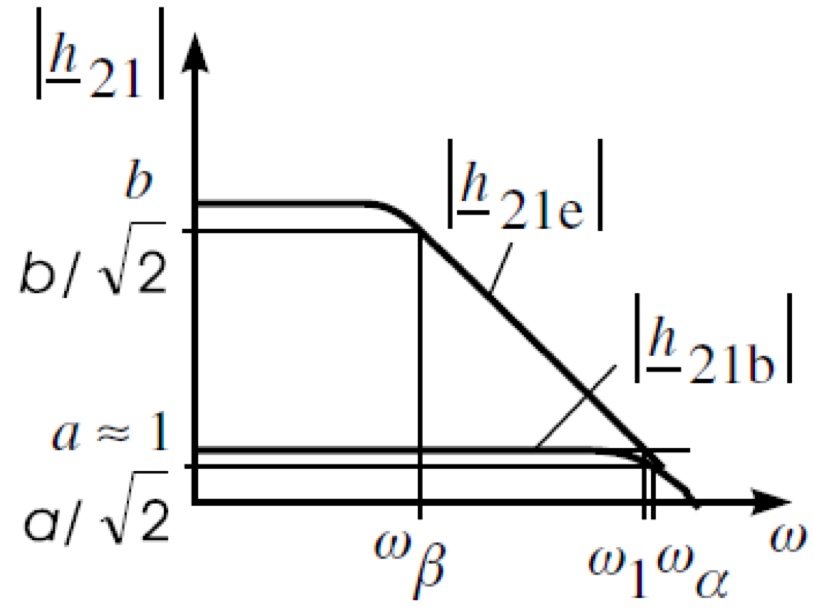
\includegraphics[width=3cm]{./bilder/BipTraFrequenzgang.png}
        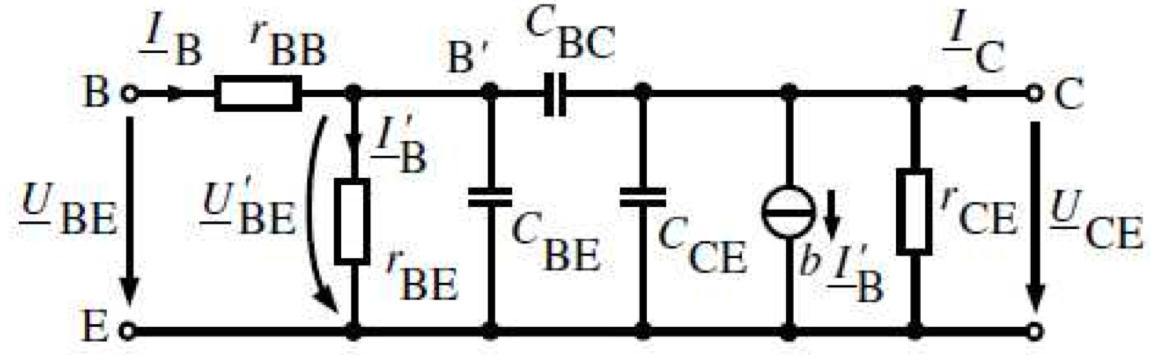
\includegraphics[width=5cm]{./bilder/BipTraErsatzschFreq.png}
      \end{minipage}
            
  \subsubsection{Temperaturverhalten von Bipolartransistoren}
    Temperaturabhängigkeit von $V_{BE}: -2mV/K$ und somit Verdoppelung des Sperrstromes bei Temperaturerh\"ohung um $10K$\\
    \begin{tabular}{ll}
      Stromverst\"arkungsfaktor &
      \fbox{$B_N(T) = B_N(T_0)\cdot e^{C_b\cdot(T-T_0)}$ mit $C_b \approx 0.6\% \cdot K^{-1}$}\\
      
      Thermischer Widerstand &
      \fbox{$P_{Vmax} = \frac{T_{max} - T_U}{R_{th}}$} \newline
      mit $R_{th} = 0.25K/mW \rightarrow$ für TO-92 Plastikgehäuse \\
    \end{tabular}
    \vspace{2mm}\hrule
    
  

  \subsubsection{Transistor als Schalter}
    \begin{minipage}[T]{13cm}
      Bei der Verwendung des Transistors als Schalter berechnet man den Basisstrom aufgrund des erforderlichen Kollektorstromes und dem           
      vorhandenen Stromverst\"arkungsfaktor und vergr\"ossert den Basisstrom dann anschliessend noch um den Faktor 2 bis 5. Dadurch wird    
      erreicht, dass der Transistor auf jeden Fall v\"ollig durchgeschaltet wird.
    \end{minipage}
    \begin{minipage}[T]{6cm}
      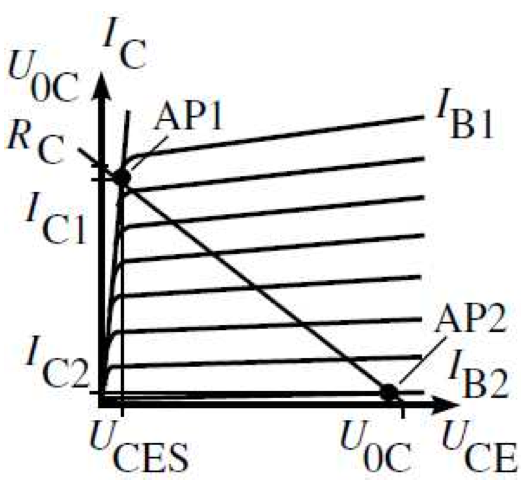
\includegraphics[height=3cm]{./bilder/BipTrAlsSchalterKennl.png}
      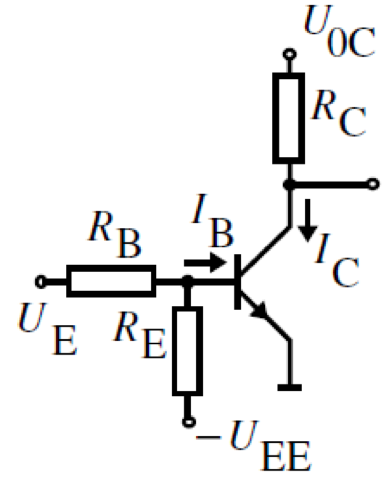
\includegraphics[height=3cm]{./bilder/BipTrAlsSchalter.png}
    \end{minipage}
            
  \subsubsection{Gegenkopplungsschaltungen zur Reduktion der Abh\"angigkeit von Temperatur und Tolleranzen}
    \begin{minipage}[T]{5.4cm}
      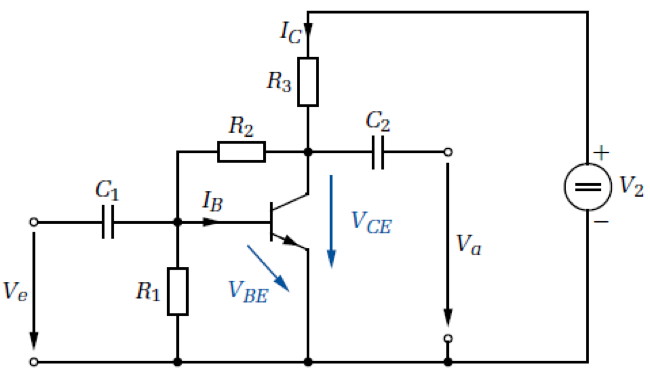
\includegraphics[height=3cm]{./bilder/Spannungsgegenkopplung.png}\\
      Spannungsgegenkopplung
    \end{minipage}
    \begin{minipage}[T]{4cm}
      Gegenkopplung durch $R_2$
    \end{minipage}
    \vrule \hspace{0.1cm}
    \begin{minipage}[T]{5.5cm}
      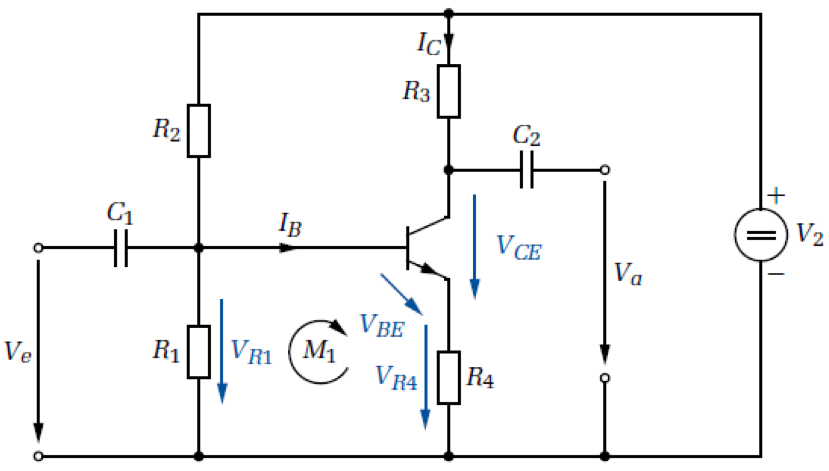
\includegraphics[height=3cm]{./bilder/Stromgegenkopplung.png} \\
      Stromgegenkopplung
    \end{minipage}
    \begin{minipage}[T]{4cm}
      Gegenkopplung durch $R_4$\\\\
      $V_{out} = -\frac{R_3}{R_4}\cdot V_{in}$\\\\
      Verst\"arkung viel kleiner als ohne Gegenkopplung
    \end{minipage}
            
  \subsubsection{Transistorverst\"arkerschaltungen}
    \begin{minipage}[T]{4.7cm}
      Emitterschaltung mit\\
      Stromgegenkopplung\\
      \includegraphics[height=3cm]{./bilder/BipTraEmitterschStGk.png}
    \end{minipage}
    \begin{minipage}[T]{4.7cm}
      Emitterschaltung mit\\
      Spannungsgegenkopplung\\
      \includegraphics[height=3cm]{./bilder/BipTraEmitterschSpGk.png}
    \end{minipage}
    \begin{minipage}[T]{5.7cm}
      Basisschaltung\\
      (Impedanzwandler)\\
      \includegraphics[height=3cm]{./bilder/BipTraBasissch.png}
    \end{minipage}
    \begin{minipage}[T]{3.7cm}
      Kollektorschaltung\\
      (Emitterfolger)\\
      \includegraphics[height=3cm]{./bilder/BipTraKollektorsch.png}
    \end{minipage}
    

  \subsection{Stromspiegel}
    \begin{minipage}{9cm}
      Spiegelverhältnis \fbox{$M = \frac{b}{b+2} = 1-\frac{2}{b+2} \approx 1$} \\
      Er spiegelt einen Referenzstrom wieder. Bei grosser Stromverstärkung ist das
      Spiegelverhältnis annähernd 1.
    \end{minipage}
    \begin{minipage}{9cm}
      \includegraphics[width=6cm]{./bilder/Stromspiegel.png}
    \end{minipage}

  \subsubsection{Differenzverst\"arker}
    \begin{minipage}[T]{11cm}
      Differenz-Verst\"arkung
      \hspace{8.4mm}\fbox{$v_d = \frac{U_{A_d}}{U_{E_d}} = -S \cdot (R_C//r_{CE}) \approx -S\cdot R_C$}\\
      Gleichtaktverst\"arkung
      \hspace{8.1mm}\fbox{$v_{gl} = -\frac{R_C}{2\cdot R_E}$}\\
      Gleichtaktunterdr\"uckung
      \hspace{3.8mm}\fbox{$G = \frac{v_d}{v_{gl}} = 2\cdot S \cdot R_E$}\\
      Ausgangsstrom
      \hspace{18.8mm}\fbox{$I_{out} = gm \cdot (V_{e1} - V_{e2})$} \\
      Transkonduktanz
      \hspace{15.6mm}\fbox{$gm = \frac{dI_{out}}{dU_{in}}$} \\
      Transimpedanz
      \hspace{19mm}\fbox{$\frac{dU_{out}}{dI_{in}}$}
    \end{minipage}
    \begin{minipage}[T]{4cm}
      S = Steilheit \\
      $U_{Ad}$ = Ausgangsdifferenz \\
      $U_{Ed}$ = Eingangsdifferenz \\
    \end{minipage}
    \begin{minipage}{4cm}
      \includegraphics[height=3cm]{./bilder/BipTraDiffAmp.png}
    \end{minipage}\\
             
    \subsubsection{Leistungsendstufen}
      \begin{minipage}[T]{4.7cm}
        Klasse A-Verst\"arker\\
        \includegraphics[height=4cm]{./bilder/KlassA_Amp.png}\\
        $\eta_{max} = \frac{P_{\sim max}}{P_=} = 25\%$
      \end{minipage}
      \begin{minipage}[T]{4.7cm}
        Klasse B-Verst\"arker\\
        \includegraphics[height=4cm]{./bilder/KlassB_Amp.png} \\
        $\eta_{max} = \frac{P_{\sim max}}{P_=} = 78.5\%$
      \end{minipage}
      \begin{minipage}[T]{4.7cm}
        Klasse AB-Verst\"arker\\
        \includegraphics[height=4cm]{./bilder/KlassAB_Amp.png}
      \end{minipage}
      \begin{minipage}[T]{4.7cm}
        Arbeitspunkte jeweiler Klassen\\\\
        \vspace{5mm}
        \includegraphics[width=4.7cm]{./bilder/EndstufenAP.png}
      \end{minipage}
      
\vspace{2mm}\hrule

\subsection{FET-Transistor}
  \subsubsection{JFET Junction Field Effect Transistor}
    \begin{minipage}[T]{8cm}
      JFET als {\bf Konstantstromquelle}:\\
      ben\"otigter Strom \fbox{$I_D = \frac{U_{GS}}{R_S}$}\\
      $U_{GS}$ entsprechend ben\"otigem Strom aus Kennlinie lesen\\
      bei der Pinch-off-Grenze (Abschn\"urgrenze) sperrt der JFET
    \end{minipage}
    \begin{minipage}[T]{3.4cm}
      \includegraphics[height=4cm]{./bilder/JFETCCQuelle.png}
    \end{minipage}
    \begin{minipage}[T]{6cm}
      \includegraphics[height=4cm]{./bilder/JFETKennlinie.png}
    \end{minipage}
    
\hrule

  \subsubsection{MOSFET Metal Oxide Silicon Field Effect Transistor}
    Thermisches Verhalten $\frac{dU_T}{dT} \approx -1 mV/K$ \\
    \begin{minipage}[T]{6cm}
      \underline{Sperrbereich}\\\\
      $V_{GS} < V_{th} \to I_D = 0$\\
      typische $V_{th} = 0.5 \ldots 1.5V$\\ 
      \includegraphics[height=4cm]{./bilder/MOSFETSperrbereich.png}
    \end{minipage}
    \begin{minipage}[T]{6cm}
      \underline{Widerstands-/Triodenbereich (linear)}\\\\
      $V_{GS} > V_{th} $ und $0 < V_{DS} \leq V_{GS} - V_{th}$\\
      $\to I_D$ fliesst\\
      \includegraphics[height=4cm]{./bilder/MOSFETLinBereich.png}
    \end{minipage}
    \begin{minipage}[T]{6cm}
      \underline{S\"attigungs-/Pentodenbereich}\\\\
      $0 < V_{GS} - V_{th} \leq V_{DS}$, mit $V_{GS} > V_{th}$ Kanal wird abgeschn\"urt\\
      \includegraphics[height=4cm]{./bilder/MOSFETSaettBereich.png}
    \end{minipage}\\
            
  \subsubsection{Steuerkennlinien von verschiedenen MOSFETs}
    \begin{minipage}[T]{9cm}
      \includegraphics[height=2.4cm]{./bilder/MOSFETSteuerkennlinien.png}
    \end{minipage}
    \begin{minipage}[T]{9cm}
      a) n-Kanal Anreicherungs-Typ (selbstsperrend)\\
      b) n-Kanal Verarmungs-Typ (selbstleitend)\\
      c) p-Kanal Anreicherungs-Typ (selbstsperrend)\\
      d) p-Kanal Verarmungs-Typ (selbstleitend)\\
    \end{minipage}
                
  
      
  \subsubsection{Berechnung des Drainstromes $I_D$}
    \begin{minipage}{13cm}
      $I_D = \begin{cases}
        0 & $f\"ur $ V_{GS} \leq V_{th}\\
        {\bf Sperrbereich}\\\\
        
        \beta\cdot(2(V_{GS}-V_{th})V_{DS} - V_{DS}^2)\cdot(1 + \lambda\cdot V_{DS}) &  $f\"ur $ 0 < V_{DS} \leq V_{GS}-V_{th},\\
        {\bf Triodenbereich} $ TB linearer Bereich$ & V_{GS} > V_{th}\\ \\
        
        \beta\cdot(V_{GS} - V_{th})^2\cdot(1 + \lambda\cdot V_{DS})    &  $f\"ur $ 0\leq V_{GS} - V_{th} \leqq V_{DS}\\
        {\bf Pentodenbereich} $ PB S\"attigungsbereich $\\
      \end{cases}$\\
                
      \begin{tabular}[t]{l l l}
        $b$: Kanalbreite & $L$: Kanall\"ange & $\mu_n$: Leitf\"ahigkeit Kanal\\
        $\epsilon_{ox}$: Dielektrizit\"at Oxidschicht & $\lambda$: Pinch-off-Konstante & $d_{ox}$: Oxiddicke\\
        $V_{th}$: Threshold-Spannung & $\beta$: Steilheitsparameter & $K$: Steilheitskoeffizient
      \end{tabular}
    \end{minipage}
    \vrule \hspace{0.1cm}
    \begin{minipage}[T]{6cm}
      \includegraphics[width=6cm]{./bilder/MOSFET_IU_Kennlinie.png}\\
      \vspace{0.8cm}\\
      Steilheitsparameter \hspace{1mm}\fbox{$\beta = \frac{K}{2} = \frac{\mu_n \epsilon_{ox}}{2d_{ox}}\frac{b}{L}$}
    \end{minipage}\\
            
  \subsubsection{Kleinsignalmodell des MOSFET}
    \begin{minipage}[T]{10.5cm}
      Steilheit
      \hspace{29.3mm}\fbox{$g_m = 2\beta(V_{GS}-V_{th}) = \sqrt{4\beta\cdot I_D}$}\\
      Ausgangsleitwert
      \hspace{15.9mm}\fbox{$g_d = \beta\lambda(V_{GS}-V_{th})^2$}\\
      Drain-Source-Widerstand
      \hspace{3mm}\fbox{$r_{DS} = \frac{1}{\lambda\cdot I_{D0}}$}\\
      Gate-Source-Spannung
      \hspace{7mm}\fbox{$V_{GS} \cong \sqrt{\frac{I_D}{\beta}} + V_{th}$}
    \end{minipage}
    \begin{minipage}[T]{3.5cm}
      \includegraphics[width=3cm]{./bilder/MOSFET_Aufbau.png}
    \end{minipage}
    \begin{minipage}[T]{5cm}
      \includegraphics[width=5cm]{./bilder/MOSFET_Ersatzsch.png}
    \end{minipage}
    
\vspace{1mm}\hrule

  \subsubsection{Differenzverst\"arker}
    \begin{minipage}[T]{14cm}
      Ausgangswiderstand
      \hspace{10.6mm}\fbox{$r_{out} = R//r_{DS}$}\\
      Verst\"arkung
      \hspace{23.3mm}\fbox{$A_D = -S \cdot (R_D//r_{DS}) \approx -S \cdot R_D$}\\
      Ausgansdifferenzspannung
      \hspace{1.7mm}\fbox{$V_{A} = A \cdot V_{D}$}
                
    \end{minipage}
    \begin{minipage}[T]{5cm}
      \includegraphics[height=4cm]{./bilder/MOSFET_Diffamp.png}
    \end{minipage}
\endgroup
\section{Referenzspannungen} 


\subsection{Verschiedene Arten der Rerferenzspannungserzeugung} 
	\begin{longtable}{|l|l|l|}
	\hline
		\begin{minipage}{4cm}
			\textbf{Einfachste "`Referenzspannungsquelle"'}
		\end{minipage}
	&
		\begin{minipage}{6cm}
			\includegraphics[width=6cm,trim=0 0 0 -5]{./bilder/spannungsteiler}
		\end{minipage}
	&
		\begin{minipage}{8cm}
			\begin{equation*}
				S_{V_{DD}}^{U_{Ref}}=\frac{\frac{\Delta
				U_{Ref}}{U_{Ref}}}{\frac{\Delta V_{DD}}{V_{DD}}}=1
			\end{equation*}
			S: Sensitivität: Relative Änderung des Ausgangs zu Relativer Änderung des Eingangs
		\end{minipage}
	\\ \hline
		\begin{minipage}{4cm}
			\textbf{Dioden Referenz}
		\end{minipage}
	&
		\begin{minipage}{6cm}
			\includegraphics[width=6cm]{./bilder/DiodenRef.png}
		\end{minipage}
	&
		\begin{minipage}{8cm}
			\begin{gather*}
				U_{Ref}=U_{EB}=\frac{kT}{e}\ln{\frac{I}{I_{s}}} \notag\\
				\text{ für }V_{DD} \gg U_{EB}\\
				S_{V_{DD}}^{U_{Ref}}=\frac{1}{\ln{\frac{I}{I_{S}}}}<1
			\end{gather*}
		\end{minipage}
	\\ \hline
		\begin{minipage}{4cm}
			\textbf{MOSFET Referenz}
		\end{minipage}
	&
		\begin{minipage}{6cm}
			\includegraphics[width=2.5cm,trim=0 0 0 -5]{./bilder/mosfetReferenz}
		\end{minipage}
	&
		\begin{minipage}{8cm}
			\begin{equation*}
				V_{REF}\approx \frac{R_{1}+R_{2}}{R_{2}}V_{GS}
			\end{equation*}
			\begin{equation*}
				V_{GS} \approx \text{ konst.}\quad\Leftrightarrow\quad V_{out} \text{ konst.}
			\end{equation*}
			$V_{GS}$ hat grosse Toleranzen $\Leftrightarrow$ eher unüblich
		\end{minipage}
	\\ \hline
		\begin{minipage}{4cm}
			\textbf{Bootstrap Referenz}
		\end{minipage}
	&
		\begin{minipage}{6cm}
			\includegraphics[width=6cm]{./bilder/bootstrapReferenz}
		\end{minipage}
	&
		\begin{minipage}{8cm}
			\begin{gather*}
				I_{1}=I_{2} \\
				I_2 \cdot R = m \cdot  U_T \cdot \ln\left(\frac{I_1}{I_S}\right) \\
				U_{T}=\frac{kT}{q}
			\end{gather*}
				Stromspiegel (PTAT-Stromquelle) \\
				(PTAT: Proportional To Absolute Temperature)
			\end{minipage}
	\\ \hline
		\begin{minipage}{4cm}
			\textbf{Bandgap Referenz}
		\end{minipage}
	&
		\begin{minipage}{6cm}
			\includegraphics[width=6cm,trim=0 0 0 -5]{./bilder/bandgapReferenz1}\\
			\includegraphics[width=6cm]{./bilder/bandgapReferenz2}
		\end{minipage}
	&
		\begin{minipage}{8cm}
			Addition aus zwei Spannungen mit umgekehrten, 
			gleich grossen Temperatur-Koeffizienten:
			\begin{enumerate}
				\item Diodenspannung mit $-2 \frac{mV}{K}$ (hier: $U_{BE3}$)
				\item PTAT-Quelle mit $V_T=\frac{kT}{q} \Rightarrow +0.085 \frac{mV}{K}$
			\end{enumerate}

			\textbf{Herleitung:} \\
			Generell ist $I_C = B \cdot I_{BS} \left(e^{\frac{U_{BE}}{U_T}} -1 \right)
							\approx B \cdot I_{BS} \cdot e^{\frac{U_{BE}}{U_T}}$ \\
			Damit wird $\frac{I_{C1}}{I_{C2}}$ zu $e^{\frac{U_{BE1}-U_{BE2}}{U_T}}$ \\
			und $\Delta U_{BE} = U_{BE1}-U_{BE2} = U_T \ln\left(\frac{I_{C1}}{I_{C2}}\right)$ \\
			\\
			Ist das Verhältnis \smash{$\frac{I_{C1}}{I_{C2}}$} konstant, was beim Stromspiegel
			erfüllt ist, so hängt $\Delta U_{BE}$ wegen \smash{$U_T=\frac{k \cdot T}{q}$} nur 
			von der absoluten Temperatur $T$ ab ist somit eine PTAT-Quelle. \\
			\\
			Weil $I_{R3} \approx I_{R2}$ hängt auch $U_{PTAT}=I_{R3} \cdot R_3$ nur von der
			absoluten Temperatur $T$ und ist somit eine PTAT-Quelle. \\
			\\
			$U_{Ref} = U_{PTAT} + U_{BE3}$ ist also die Addition einer PTAT-Quelle und einer
			Diodenspannung und somit praktisch temperaturunabhängig mit 
			$U_{Ref} \stackrel{!}{\approx} 1,2V$. \\
			\\
			\textit{Oft als integrierte Bauteile erhältlich.}
		\end{minipage}
	\\ \hline
		\begin{minipage}{4cm}
			\textbf{Zenerdiode Referenz}
		\end{minipage}
	&
		\begin{minipage}{6cm}
			\includegraphics[width=6cm,trim=0 0 0 -5]{./bilder/zenerReferenz}
		\end{minipage}
	&
		\begin{minipage}{8cm}
			Häufigste Spannung: $5,6V$ (minimaler Temperaturkoeffizient)
		\end{minipage}
	\\ \hline
\end{longtable}


\begingroup
  \let\clearpage\relax
  \section{Spannungsregler}
  {\bf{Qualit\"atsmasse}}\\
  \begin{minipage}[t]{6cm}
    Ausg.-spannung bestimmt durch:\\
    relativen Stabilisierungsfaktor $S'$\\
    \vspace{0.5mm}{$S' = \frac{\frac{\Delta U_e}{U_e}}{\frac{\Delta U_a}{U_a}}$}
  \end{minipage}
  \begin{minipage}[t]{6cm}
    Temperaturverhalten:\\
    Temperaturkoeffizient $TK_U$\\
    \vspace{0.5mm}{$TK_U = \frac{1}{U_a}\frac{dU_a}{dT}$}
  \end{minipage}
  \begin{minipage}[t]{6cm}
    Lastabh\"angigkeit:\\
    dynamischer Ausgangswiderstand $r_a$\\
    \vspace{0.5mm}{$r_a = \frac{dU_a}{dI_a}$}
  \end{minipage}\\ 
    
\subsection{Linearer Regler}
  \begin{minipage}[T]{14cm}
    Ausgangsspannung
    \hspace{13mm}\fbox{$V_{out} = \left(1+\frac{R_1}{R_2}\right) \cdot V_{ref}$}\\
  \end{minipage}
  \begin{minipage}{5cm}
    \includegraphics[height=1.5cm]{./bilder/ReglerLinear.png}
  \end{minipage}\\
            
\subsection{Einstellbarer Regler}
  \begin{minipage}[T]{14cm}
    Ausgangsspannung
    \hspace{13mm}\fbox{$V_{out} = V_{ref} + R_2 \cdot\left(\frac{V_{ref}}{R_1} + I_{adj}\right)  \approx\left(1+\frac{R_2}{R_1}\right) 
    \cdot V_{ref}$}\\
  \end{minipage}
  \begin{minipage}{5cm}
    \includegraphics[height=2.5cm]{./bilder/ReglerEinstellbar.png}
  \end{minipage}\\
        
\subsection{Aufw\"artswandler (Step up, Boost)}
  \begin{minipage}[T]{14cm}
    Lade-Phase (S geschlossen)
    \hspace{0.5mm}\fbox{$\Delta I_{L\_on} = \frac{1}{L}V_{in}\cdot t_{on}$}\\  
    Entlade-Phase (S offen)
    \hspace{5.8mm}\fbox{$\Delta I_{L\_off} = \frac{1}{L}(V_{in}-V_{out})\cdot t_{off}$}\\  
    Gleichgewicht
    \hspace{21mm}\fbox{$\Delta I_{L\_on} =-\Delta I_{L\_off}$}\\  
    Ausgangsspannung
    \hspace{13mm}\fbox{$V_{out} = V_{in}\cdot \left(1+\frac{t_{on}}{t_{off}}\right)$}\\
  \end{minipage}
  \begin{minipage}{5cm}
    \includegraphics[width=4cm]{./bilder/ReglerStepUpStromverlauf.png}
  \end{minipage}\\
        
\subsection{Abw\"artswandler (Step Down, Buck)}
  \begin{minipage}[T]{14cm}
    Lade-Phase (S geschlossen)
    \hspace{0.5mm}\fbox{$\Delta I_{L\_on} = \frac{1}{L}\int_{0}^{T_i}{(V_{in}-V_{out})dt} = \frac{1}{L}(V_{in}-V_{out})\cdot T_i$}\\  
    Entlade-Phase (S offen)
    \hspace{5.8mm}\fbox{$\Delta I_{L\_off} = \frac{1}{L}\int_{T_i}^{T_S}{(V_{out}+V_{D_f})dt}= \frac{1}{L}(V_{out}+V_{D_f})(T_S-T_i)$}\\
    Ausgangsspannung
    \hspace{13mm}\fbox{$V_{out} = \frac{T_i}{T_S}\cdot V_{in} - \left(1-\frac{T_i}{T_S}\right) \cdot V_{D_f} \approx \frac{T_i}{T_S}
    \cdot V_{in}$}\\
  \end{minipage}
  \begin{minipage}{5cm}
    \includegraphics[width=5cm]{./bilder/ReglerStepDown.png}
  \end{minipage}\\
        
\subsection{Invertierender Wandler (Buck-Boost)}
  \begin{minipage}[T]{8cm}
    Ausgangsspannung
    \hspace{13mm}\fbox{$V_{out} = -\frac{T_i}{T_S}\cdot V_{in}$}\\
  \end{minipage}
  \begin{minipage}{6cm}
    $T_i$ = Einschaltzeit\\
    $T_s$ = Ausschaltzeit
  \end{minipage}
  \begin{minipage}{5cm}
    \includegraphics[width=4cm]{./bilder/ReglerInvert.png}
  \end{minipage}\\
        
\subsection{Ladepumpen (Charge-Pumps)}
  \begin{minipage}[T]{14cm}
    \hspace*{43.3mm}\fbox{$\Delta V_{out} = \frac{\Delta Q_1}{C_1+C_L} = \frac{C_1(V_{in}-V_{out})}{C_1+C_L} = \frac{V_{in}-V_{out}}{1+
    \frac{C_L}{C_1}}$}\\
    \hspace*{43.3mm}\fbox{$\Delta Q = C_L \cdot \Delta V_{out} = \frac{C_1 C_L}{C_1+C_L}(V_{in}-V_{out})$}\\
    \hspace*{43.3mm}\fbox{$I_{out} = \frac{\Delta Q}{T_S} = \frac{C_1 C_L}{C_1+C_L}\frac{V_{in}-V_{out}}{T_S}$}\\
    \hspace*{43.3mm}Ver\"anderung der Ausgangsspannung durch ver\"andern der\\
    \hspace*{43.3mm}Schaltfrequenz
  \end{minipage}
  \begin{minipage}{5cm}
    \includegraphics[width=5cm]{./bilder/ReglerChargePump.png}
  \end{minipage}\\  
    
\newpage

\subsection{Wichtiges zu Spule / Kondensator}
  Energie im Mag.-Feld
  \hspace{9mm}\fbox{$W_m = \frac{1}{2} \cdot L \cdot I^2 = \frac{1}{2}\cdot N \cdot I \cdot \Phi$}\\
  Energie im El.-Feld
  \hspace{12.5mm}\fbox{$W_E = \underbrace{\frac{1}{2} \cdot C \cdot U^2}_{U = konst}  = \frac{1}{2} \cdot Q \cdot U = \underbrace{\frac{1}{2}
  \cdot\frac{Q^2}{C}}_{Q = konst}$}\\
  Spule
  \hspace{34mm}\fbox{$u_L(t) = L \cdot \frac{di(t)}{dt}$}\\
  \hspace*{43.5mm}\fbox{$i_L(t) = \frac{1}{L}\int\limits_0^t u(\tau)d\tau + i(0)$}\\
  Kondensator
  \hspace{22.7mm}\fbox{$u_C(t) = \frac{1}{C}\int\limits_0^t i(\tau)d\tau + u(0)$}\\
  \hspace*{43.5mm}\fbox{$i_C(t) = C \cdot \frac{du(t)}{dt}$}\\
     
  \section{Oszillatoren}
\subsection{Typen}
	\begin{center}
		\includegraphics[width=11cm]{./bilder/OszillatorKlassifikation.png}
	\end{center}

\subsection{Untuned Oscillators}
	\subsubsection{Astabiler Multivibrator mit Transistor}
	\begin{minipage}{6cm}
		\includegraphics[width=6cm]{./bilder/multiVibrator}
	\end{minipage}
	\begin{minipage}{10cm}
		$t_1 = t_2 = 0.7 \cdot 100k\Omega \cdot 100\mu F$ \\
		$T = t_1 + t_2$
	\end{minipage}

\subsubsection{Astabiler Multivibrator mit Komparator}
	\begin{multicols}{3}
		\includegraphics[width=6cm]{./bilder/osziRechteck.png}
		\columnbreak
		
		\includegraphics[width=6cm]{./bilder/osziRechteckSignal.png}
		\columnbreak
		
		$V_{T+}=V_{outMAX}\cdot\frac{R_2}{R_2+R_3}$\\
		$V_{T-}=V_{outMIN}\cdot\frac{R_2}{R_2+R_3}$\\
		$V_c(t)=V_{T-}+\left(V_{outMAX}-V_{T-}\right)\left(1-e^{\frac{-t}{R_1\cdot
		C_1}}\right)$\\
		$f=\frac{1}{T}=\frac{1}{2R_1C_1 ln \frac{R_3+2R_2}{R3}}$\\
		wenn: $R2 = 0.86 \cdot R_3$ dann gilt:\\
		$f=\frac{1}{2\cdot R_1C_1}$
	\end{multicols}
\subsubsection{Dreieck Rechteck Generator}
	\begin{multicols}{3}
		\begin{center}
			\includegraphics[width=3.5cm]{./bilder/osziDreieckRechteckBlock.png}\\
		\end{center}
		\includegraphics[width=6cm]{./bilder/osziDreieckRechteck.png}
		\columnbreak
		
		\includegraphics[width=6cm]{./bilder/osziDreieckRechteckSignal.png}
		\columnbreak
			
		$V_2\left(t\right)=-\frac{1}{R_1C}\int V_1\left(t\right)dt+V_{2 Anfang}$\\
		$V_H=2\left|V_T\right|=\left(V_{outMAX}-V_{outMIN}\right)\frac{R_2}{R_3}$\\
		$T=\frac{2\cot V_H \cdot R_1C}{V_{outMAX}}$\\
	\end{multicols}
\subsubsection{Kippschaltung}
	\begin{minipage}{9cm}
		\includegraphics[width=9cm]{./bilder/kippschaltung}
	\end{minipage}
	\begin{minipage}{6cm}
		$\tau = R \cdot C $\\
		$T_1 = \tau \cdot \ln \left(\frac{U_{AH}-U_{SL}}{U_{AH}-U_{SH}} \right)$ \\
		$T_2 = \tau \cdot \ln \left(\frac{U_{SH}-U_{AL}}{U_{SL}-U_{AL}} \right)$ \\
		$f = \frac{1}{T_1 + T_2}$
	\end{minipage}
\subsubsection{Ringoszilatoren}
	\begin{multicols}{3}
	 	\includegraphics[width=6cm]{./bilder/osziRing.png} \\
    Oszillatorfrequenz \fbox{$f_{OSC} = \frac{1}{2\cdot n \cdot t_g}$} \\
    $t_g$: Time-Delay pro Inverter\\
    $n$: ungerade Anzahl Inverter\\
		\columnbreak
		
		\includegraphics[width=6cm]{./bilder/osziRingSignal.png}	
		\columnbreak
		
		\includegraphics[width=6cm]{./bilder/osziRingCMOS.png}
	\end{multicols}
	
\subsection{Tuned Oscillators}
	Oszillatoren mit Rückkopplung. Schwingbedingung: Verstärkung im gesamten Kreis $=1$. 
	\subsubsection{LC-Oszillator}
		\begin{multicols}{2}
			\textbf{Normaler LC-Oszillator} \\
			\includegraphics[width=6cm]{./bilder/lcOszillator}
			
		\columnbreak
			$U_2(t) = (1+\frac{R_2}{R_1}) \cdot U_1(t) = V_u \cdot U_1(t)$ \\
			
			Daraus folgt die Schwingungsgleichung \\
			$\frac{d^2 U_1(t)}{dt^2}+2k\omega_0 \frac{dU_1(t)}{dt}+\omega^2U_1(t)=0$ \\
			
			und \\
			$\omega_0 = \frac{1}{\sqrt{L\cdot C}}$
		\end{multicols}
		
		\begin{multicols}{2}
			\textbf{Colpitts-Oszillator}\\
			\includegraphics[width=6cm]{./bilder/osziLC.png}\\
			
		\columnbreak
		
			$\omega_0=\frac{1}{\sqrt{L\frac{C_1 C_2}{C_1+C_2}}}$\\
			
		\end{multicols}

	\subsubsection{Quarz-Oszilator}
		\begin{tabular}{lll}
			\textbf{Ersatzschaltung} & \textbf{Phasengang} & \textbf{Anwendung} \\
			\begin{minipage}{6cm}
				\includegraphics[width=3cm]{./bilder/osziCrystal.png}
			\end{minipage} &
			\begin{minipage}{6cm}
				\includegraphics[width=5cm]{./bilder/quarz-kennl.png}
			\end{minipage} & 
			\begin{minipage}{6cm}
					\includegraphics[width=5cm]{./bilder/quarz-schaltung.png}
			\end{minipage}	\\
		\end{tabular}	
			
		Frequenzabweichung: $\frac{\Delta f}{f_0} \approx 10^{-6} \dots 10^{-10}$ \\
		
	\subsection{Spannungsgesteuerte Oszillatoren (VCO)}
		\begin{minipage}{12cm}
			\includegraphics[width=12cm]{./bilder/vco.png}
		\end{minipage}
		\begin{minipage}{6cm}
			$f_{osc} = \frac{R_1 + R_2}{4 R_1} \cdot \frac{1}{RC} \cdot \frac{U_{ctrl}}{|U_{out}|}$ \\
			
			was vereinfacht wird zu \\
			$f_{osc} = K_{VCO} \cdot U_{ctrl}$ mit $K_{VCO}$ als konstantem Faktor.
		\end{minipage}
\endgroup


\end{document}

